\documentclass[12pt,spanish,Letterpaper,openany]{book}
\usepackage{lmodern}
\usepackage{setspace}
\setstretch{0.85}
\usepackage{amssymb,amsmath}
\usepackage{ifxetex,ifluatex}
\usepackage{fixltx2e} % provides \textsubscript
\ifnum 0\ifxetex 1\fi\ifluatex 1\fi=0 % if pdftex
  \usepackage[T1]{fontenc}
  \usepackage[utf8]{inputenc}
\else % if luatex or xelatex
  \ifxetex
    \usepackage{mathspec}
  \else
    \usepackage{fontspec}
  \fi
  \defaultfontfeatures{Ligatures=TeX,Scale=MatchLowercase}
    \setmainfont[Scale=1.0, HyphenChar=None]{Corbel}
    \setsansfont[]{Corbel}
    \setmonofont[Mapping=tex-ansi]{Corbel}
\fi

\makeatletter
\renewcommand\mainmatter{\clearpage\@mainmattertrue\pagenumbering{arabic}}
\renewcommand\frontmatter{\clearpage\@mainmatterfalse\pagenumbering{arabic}}
\renewcommand\backmatter{\clearpage\@mainmatterfalse}
\makeatother

%\usepackage{etoolbox}
%\makeatletter
%\patchcmd{\@smemmain}{\cleardoublepage}{\clearpage}{}{}
%\patchcmd{\@smemmain}{\cleardoublepage}{\clearpage}{}{}
%\patchcmd{\@smemfront}{\cleardoublepage}{\clearpage}{}{}
%\patchcmd{\@smemfront}{\cleardoublepage}{\clearpage}{}{}
%\makeatother

\setlength{\parindent}{0em}

\usepackage{graphicx}
\usepackage{booktabs}
\usepackage{multicol}
\usepackage{doc}
\usepackage{float}
\usepackage{tcolorbox} 
\usepackage{lipsum}
\usepackage{tikz}
\usepackage{nonfloat}

\usepackage{pdfpages}

\usepackage[
contents={},
opacity=1,
scale=1.5,
color=blue!90
]{background}
\usepackage{lipsum}
\usepackage{ifthen}

\usepackage{xcolor}
\usepackage[pagestyles]{titlesec}

\renewpagestyle{plain}[\normalsize\sffamily\bfseries\slshape]{
  \setfoot{}{\color{white}{\thepage}}{}}

\newpagestyle{myps}[\normalsize\sffamily\bfseries\slshape]{
  \setfoot{}{\color{white}{\thepage}}{}}
  
\pagestyle{myps}


\usepackage{framed}
\definecolor{colorlinetitle}{HTML}{a3C17C}%{A2C27C}%
\definecolor{textlinetitle}{HTML}{001077}%{25408F}%{243F8E}%
\definecolor{fondo}{HTML}{DCEEA7}%
\definecolor{newfondo}{HTML}{D9E6CA}%
\colorlet{shadecolor}{fondo!81!}


% use upquote if available, for straight quotes in verbatim environments
\IfFileExists{upquote.sty}{\usepackage{upquote}}{}
% use microtype if available
\IfFileExists{microtype.sty}{%
\usepackage{microtype}
\UseMicrotypeSet[protrusion]{basicmath} % disable protrusion for tt fonts
}{}
\usepackage[inner=12.7mm,outer=12.7mm,top=25mm,bottom=21.0mm]{geometry}
\usepackage{hyperref}
\hypersetup{unicode=true,
            pdftitle={Revista de la Unidad de Prácticas de Ingeniería y EPS},
            pdfauthor={Unidad de Prácticas de Ingeniería y EPS},
            pdfborder={0 0 0},
            breaklinks=true}
\urlstyle{same}  % don't use monospace font for urls
\ifnum 0\ifxetex 1\fi\ifluatex 1\fi=0 % if pdftex
  \usepackage[shorthands=off,main=spanish]{babel}
\else
  \usepackage{polyglossia}
  \setmainlanguage[]{spanish}
\fi
\usepackage{natbib}
\bibliographystyle{apalike}
\usepackage{longtable,booktabs}
\usepackage{graphicx,grffile}
\makeatletter
\def\maxwidth{\ifdim\Gin@nat@width>\linewidth\linewidth\else\Gin@nat@width\fi}
\def\maxheight{\ifdim\Gin@nat@height>\textheight\textheight\else\Gin@nat@height\fi}
\makeatother
% Scale images if necessary, so that they will not overflow the page
% margins by default, and it is still possible to overwrite the defaults
% using explicit options in \includegraphics[width, height, ...]{}
\setkeys{Gin}{width=\maxwidth,height=\maxheight,keepaspectratio}
\IfFileExists{parskip.sty}{%
\usepackage{parskip}
}{% else
\setlength{\parindent}{0pt}
\setlength{\parskip}{6pt plus 2pt minus 1pt}
}
\setlength{\emergencystretch}{3em}  % prevent overfull lines
\providecommand{\tightlist}{%
  \setlength{\itemsep}{0pt}\setlength{\parskip}{0pt}}
\setcounter{secnumdepth}{5}
% Redefines (sub)paragraphs to behave more like sections
\ifx\paragraph\undefined\else
\let\oldparagraph\paragraph
\renewcommand{\paragraph}[1]{\oldparagraph{#1}\mbox{}}
\fi
\ifx\subparagraph\undefined\else
\let\oldsubparagraph\subparagraph
\renewcommand{\subparagraph}[1]{\oldsubparagraph{#1}\mbox{}}
\fi

%%% Use protect on footnotes to avoid problems with footnotes in titles
\let\rmarkdownfootnote\footnote%
\def\footnote{\protect\rmarkdownfootnote}


  \title{Revista de la Unidad de Prácticas de Ingeniería y EPS}
    \author{Unidad de Prácticas de Ingeniería y EPS}
      \date{2020-09-22}

% no title page
\AtBeginDocument{\let\maketitle\relax}

\usepackage{caption}
\captionsetup{%
labelsep=colon,%
font={footnotesize},%
aboveskip=0.5\baselineskip,%
belowskip=0\baselineskip,% deve essere 0 perché regolo lo spazio dal testo con \intextsep
}%


\usepackage{booktabs}
\usepackage{longtable}

\usepackage{indentfirst}
\setlength{\parindent}{1em}
\usepackage{enumitem}
\setlist[itemize]{labelindent = \parindent, leftmargin=*}

%\usepackage{framed,color}
%\definecolor{shadecolor}{RGB}{248,248,248}

\renewcommand{\textfraction}{0.05}
\renewcommand{\topfraction}{0.8}
\renewcommand{\bottomfraction}{0.8}
\renewcommand{\floatpagefraction}{0.75}

\renewcommand{\chaptername}{Artículo}
\addto\captionsspanish{\renewcommand{\chaptername}{Artículo}}
\addto\captionsspanish{\renewcommand{\contentsname}{Índice General}}


\frenchspacing
\tolerance=5000
\multicoltolerance=3000 

\raggedbottom
\raggedcolumns

\setlength{\columnsep}{1em}
%We want a rule between columns.
%\setlength\columnseprule{.4pt}

%Tambien queremos asegurarnos de que un nuevo entorno multicols 
%encuentre suficiente espacio en la parte inferior de la pagina.
\setlength\premulticols{6\baselineskip}

%Al equilibrar columnas, ignoramos las soluciones que son 
%demasiado malas. Ademas, si la ultima columna es demasiado mala, 
%la tipeamos sin estirar.
\setcounter{columnbadness}{7000}
\setcounter{finalcolumnbadness}{7000}

\newcommand{\prefacetitlecommand}%
{\titleformat{\chapter}[display]%
{\bfseries\large\color{colorlinetitle}}%
{\relax}%
{0ex}%
{{\titlerule[1.2pt]}\filright\color{textlinetitle}}[\color{colorlinetitle}\vspace{0.5ex}{\titlerule[1.2pt]}]%
}


\newcommand{\articletitlecommand}%
{\titleformat{\chapter}[display]%
{\bfseries\large\color{colorlinetitle}}%
{\relax}%
{0ex}%
{{\titlerule[1.2pt]}\filright\color{textlinetitle}}[\color{colorlinetitle}\vspace{0.5ex}{\titlerule[1.2pt]}]%
}



\newcommand{\sectionCenter}%
{\titleformat{\section}[block]%
{\bfseries\large\color{textlinetitle}\filcenter}%
{\relax}%
{0ex}%
{\empty}%
}


\newcommand{\sectionRight}%
{\titleformat{\section}[block]%
{\bfseries\large\color{textlinetitle}}%
{\relax}%
{0ex}%
{\empty}%
}


\newcommand{\subsectionRight}%
{\titleformat{\subsection}[block]%
{\bfseries\normalsize\color{textlinetitle}}%
{\relax}%
{0ex}%
{\empty}%
}

\usepackage{titletoc}
\titlecontents{chapter}[3em]
{\vspace{5mm}}
{\normalsize\contentslabel[\color{textlinetitle}\thecontentslabel]{2em}\color{black}\itshape\normalsize}
{\color{black}\itshape\normalsize}
{\color{colorlinetitle}\titlerule*[.3pc]{.}\color{black}\contentspage}

\newcommand{\tcolorboxcommand}{\begin{tcolorbox}[sharp corners=uphill, colback=newfondo, colframe=newfondo, arc=6mm, boxrule=0mm, boxsep=0mm]}

\newcommand{\photocommand}[2]{%
\fcolorbox[HTML]{DCEEA7}{DCEEA7}{%
\begin{minipage}{95.19mm}%
	\hspace{1mm}%
	\begin{minipage}{22.49mm}%
		\vspace{1mm}%
		\includegraphics[width=22.49mm, height=31.96mm]{#1}%
		\vspace{1mm}%
	\end{minipage}%
	\hspace{2.4mm}%
	\begin{minipage}{68.80mm}%
		#2
	\end{minipage}%
	\hspace{0.5mm}%
\end{minipage}%
}%
}

\definecolor{fondobiography}{HTML}{DCEEA7}

\NewDocumentEnvironment{photobiography}{m O{}}%
{%
\begin{tcolorbox}[colback=fondobiography, colframe=fondobiography, width=97.19mm, boxsep=-2mm, arc=0mm]
\begin{minipage}{95.19mm}%
	%\hspace{1mm}%
	\begin{minipage}{22.49mm}%
		\vspace{2mm}%
		\includegraphics[width=22.49mm, height=31.96mm]{#1}%
		\vspace{2mm}%
	\end{minipage}%
	\hspace{2.4mm}%
	\begin{minipage}{68.80mm}%
	#2%
}%
{%
	\end{minipage}%
	%\hspace{0.5mm}%
\end{minipage}%
\end{tcolorbox}
}


\newcommand{\spacetext}{\vspace{8.1mm}}
\newcommand{\minimalspacetext}{\vspace{1mm}}
\newcommand{\spaceelevenmilis}{\vspace{11mm}}
\newcommand{\spacetenmilis}{\vspace{10mm}}
\newcommand{\spaceninemilis}{\vspace{9mm}}
\newcommand{\spaceeightmilis}{\vspace{8mm}}
\newcommand{\spacesevenmilis}{\vspace{7mm}}
\newcommand{\spacesixmilis}{\vspace{6mm}}
\newcommand{\spacefivemilis}{\vspace{5mm}}
\newcommand{\spacefourmilis}{\vspace{4mm}}
\newcommand{\spacethreemilis}{\vspace{3mm}}
\newcommand{\spacetwomilis}{\vspace{2mm}}
\newcommand{\spaceinitialeditorialcontenido}{\vspace{8.1mm}}
\newcommand{\spaceoneminus}{\vspace{-1mm}}
\newcommand{\spacetwominus}{\vspace{-2mm}}
\newcommand{\spacefourminus}{\vspace{-4mm}}

\newcommand{\HRule}{\begin{center}\rule{0.5\linewidth}{0.2mm}\end{center}}

\begin{document}
\maketitle

% \pagestyle{plain}

\includepdf{images/cover.pdf}

\AddEverypageHook{%
\ifthenelse{\value{page}<35}%
{\ifthenelse{\isodd{\value{page}}}%
  	{\backgroundsetup{scale=1, color=black, opacity=1, angle=0, contents={
\includegraphics[width=\paperwidth,height=\paperheight]{latex/background_numberimpar.pdf}}}}%
  	{\backgroundsetup{scale=1, color=black, opacity=1, angle=0, contents={
\includegraphics[width=\paperwidth,height=\paperheight]{latex/background_numberpar.pdf}}}}%
}{}%
\BgMaterial}

%%%%%%{
%%%%%%\setcounter{tocdepth}{0}
%%%\tableofcontents
%%%}
%%%%%%%%%%%%\listoffigures
%%%
\prefacetitlecommand

\titlespacing*{\chapter} {0pt}{0pt}{2pt}

\addtocontents{toc}{\vspace{3mm}~\hfill\color{textlinetitle}\textbf{Pág.}\vspace{3mm}\par}

\hypertarget{index}{%
\chapter*{Editorial}\label{index}}
\addcontentsline{toc}{chapter}{Editorial}

\begin{center}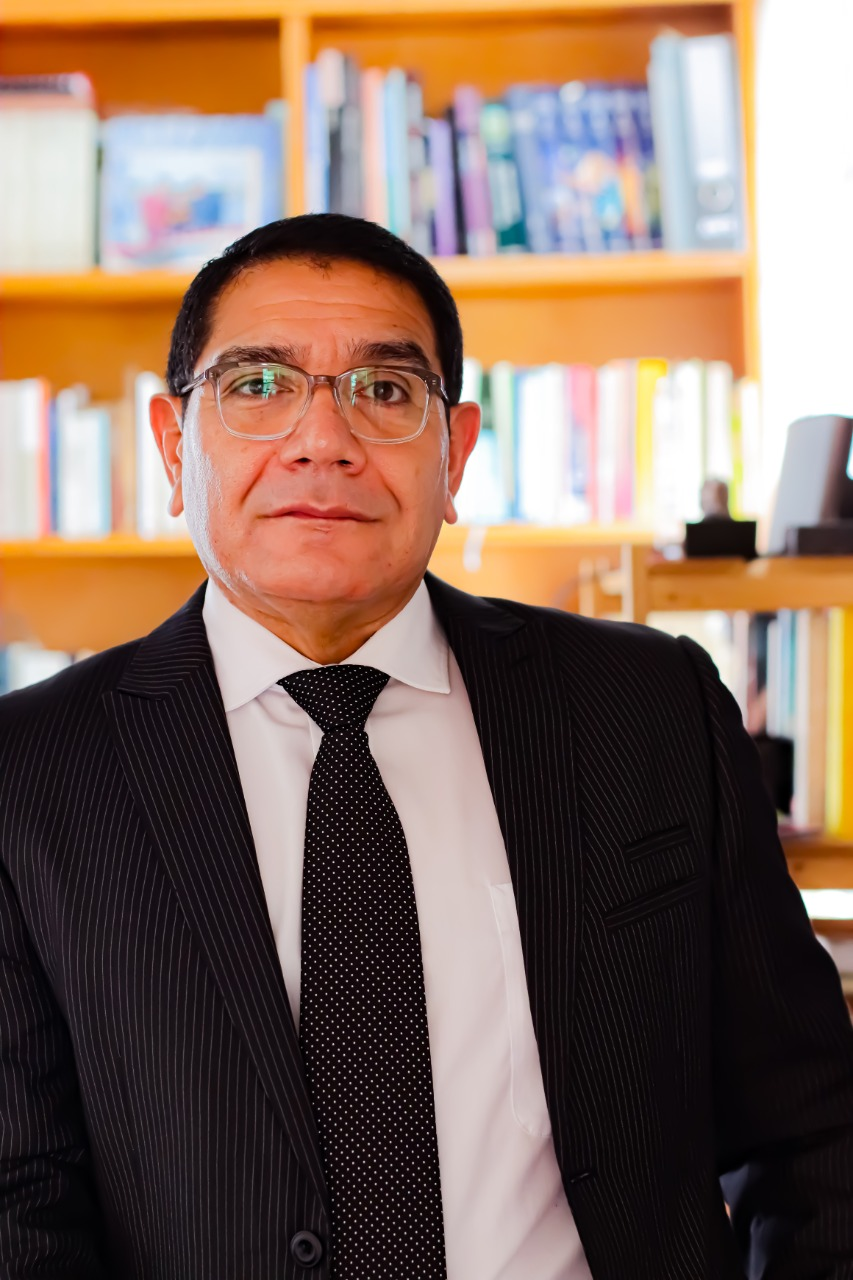
\includegraphics[width=0.27\linewidth]{images/image01_bhernandez} \end{center}

\begin {center}

\textbf{Nuevos desafíos del aprendizaje virtual en la Universidad de San Carlos}

\end {center}

A inicios de marzo, repentinamente, 190 mil estudiantes y 11 mil docentes de la Universidad de San Carlos de Guatemala nos vimos obligados a emprender una nueva aventura como consecuencia del confinamiento y distanciamiento social como medida frente a la pandemia del COVID‐19. En la Facultad de Ingeniería, los 14 mil estudiantes y 565 docentes de las carreras de grado y postgrado se enfrentaron abruptamente a entornos de aprendizaje que no habían sido planificados o avizorados; de lo presencial pasamos al mundo de la educación a distancia, fuera esta por la vía virtual o hasta por llamadas telefónicas. Las situaciones de aprendizaje para los estudiantes, a pesar de su manejo de las nuevas tecnologías de la comunicación e información, cambiaron drásticamente las rutinas. El uso de los dispositivos que otrora eran utilizados como vía de socialización o diversión, ahora se transformarían en herramientas básicas para los estudios universitarios.

Como todo cambio, las dificultades que han atravesado los estudiantes y docentes no han sido pocas. Prácticamente, todo el año 2020 las clases han ido cobrando un matiz virtual y aún no se sabe qué depara el año 2021. En todo caso, algunas de las experiencias que se viven en la USAC nos indican, entre otras, las siguientes situaciones:

En primer lugar, los docentes requerimos una capacitación profunda en andragogía o pedagogía, pues la docencia no solo radica en el conocimiento del campo, sino también y muy profundamente, demanda de capacidades de investigación y trasferencia de competencias hacia los estudiantes, según el componente teórico‐práctico que exige la profesión y la academia. Pero particular formación exige la educación a distancia y virtual que va más allá de pretender seguir haciendo frente a un dispositivo electrónico, lo que se venía realizando de manera presencial.

En segundo lugar, deben llevarse a cabo revisiones curriculares y trabajo de planificación conjunta de los docentes para dar unidad a los aprendizajes en las diferentes carreras. Al mismo tiempo, ponderar las condiciones y posibilidades de los tiempos requeridos. De hecho, el trabajo en casa tanto de docentes como de estudiantes, muchas veces aumenta y además presenta nuevas dificultades y oportunidades que no se tenían bajo la modalidad presencial.

En tercer lugar, hay que pensar en los dispositivos, plataformas, recursos y ayudas para llevar a cabo la educación en la universidad, aspecto en el cual la Facultad de Ingeniería puede jugar un papel de apoyo a otras Facultades y Escuelas por la experiencia de la plataforma UEDI, a pesar que aún quedan pendientes de la misma, concerniente a los componentes fundamentales del aprendizaje. De hecho, se reporta que hay docentes y estudiantes que solo disponen del teléfono como vía de comunicación, con lo cual su intercambio se reduce a llamadas telefónicas, whatsapp, o Facebook. Otros profesores solo utilizan los mensajes de correos electrónicos. Hay un buen porcentaje que usa las redes sociales o sistemas de almacenamiento e intercambio de información, así como también plataformas como el Zoom, Google Meet, Microsoft Teams, Ciscowebexmeet o más sofisticadas como Classroom, Moodle y otras. La universidad, en este sentido, debe realizar acciones urgentes para dar una respuesta consistente, unificada y de bajo costo a esta demanda.

En cuarto lugar, para algunos estudiantes es difícil el acceso y condiciones para concentrarse en su proceso educativo, pues muchos tienen que conectarse desde sus casas o lugares de trabajo. Su participación en los procesos de aprendizaje dependerá de la capacidad económica para pagar el ancho de banda adecuada, además de la limitación que implica compartir dispositivos con otros familiares y disponer de lugares para enfocarse en sus actividades formativas. Esto sin contar el aumento presupuestario en términos de pago de servicios como la energía eléctrica.

En quinto lugar, los recursos educativos ante la dinámica del cierre de las bibliotecas, archivos físicos y centros de práctica constituyen otro desafío para el aprendizaje. Esa relación entre investigación como parte de lo que ahora se denomina actividades asincrónicas, o trabajo independiente del estudiante, resulta también todo un esfuerzo adicional. No solo de búsqueda en el internet, sino también de formas dirigidas a través de la capacidad de acceso a un sinnúmero de recursos en línea como revistas, bases de datos bibliográficas, repositorios digitales u otros, pero que tienen un costo y que la propia universidad debería resolver. Además del diseño de medidas de seguridad y protocolos para lo que será la reinserción a la práctica profesional y uso de laboratorios.

Aún así hay que destacar el esfuerzo y buena disposición tanto de estudiantes como de profesores, para superar en esta primera fase los efectos de la pandemia del COVID‐19; a pesar de que aún queda mucho por hacer, inversiones por realizar y políticas claras que vendrían a respaldar lo que la Universidad de San Carlos y la Facultad de Ingeniería han pretendido durante los años de su existencia: una educación de calidad.

\spacefourmilis

\begin {center}

\textbf{Dr.~Bienvenido Argueta Hernández}\\
\hspace{3.2cm} Especialista en educación y currículo,
\newline asesor en temas educativos en diversas universidades a nivel nacional e internacional.

\end {center}

\medskip

\HRule

\medskip

\newpage

\hypertarget{directorio}{%
\chapter*{Directorio}\label{directorio}}
\addcontentsline{toc}{chapter}{Directorio}

\spacetwomilis

\begin{center}
\includegraphics{images/201901-logo} \end{center}
\spacetwominus

\sectionCenter

\hypertarget{nomina-de-junta-directiva}{%
\section*{Nómina de Junta Directiva}\label{nomina-de-junta-directiva}}
\addcontentsline{toc}{section}{Nómina de Junta Directiva}

\begin{longtable}[]{@{}ll@{}}
\endhead
\begin{minipage}[t]{0.239\columnwidth}\raggedright
DECANO\strut
\end{minipage} & \begin{minipage}[t]{0.35\columnwidth}\raggedright
Inga. Aurelia Anabela Córdova Estrada\strut
\end{minipage}\tabularnewline
\begin{minipage}[t]{0.239\columnwidth}\raggedright
VOCAL I\strut
\end{minipage} & \begin{minipage}[t]{0.35\columnwidth}\raggedright
Ing. José Francisco Gómez Rivera\strut
\end{minipage}\tabularnewline
\begin{minipage}[t]{0.239\columnwidth}\raggedright
VOCAL II\strut
\end{minipage} & \begin{minipage}[t]{0.35\columnwidth}\raggedright
Ing. Mario Renato Escobedo Martínez\strut
\end{minipage}\tabularnewline
\begin{minipage}[t]{0.239\columnwidth}\raggedright
VOCAL III\strut
\end{minipage} & \begin{minipage}[t]{0.35\columnwidth}\raggedright
Ing. José Milton de León Bran\strut
\end{minipage}\tabularnewline
\begin{minipage}[t]{0.239\columnwidth}\raggedright
VOCAL IV\strut
\end{minipage} & \begin{minipage}[t]{0.35\columnwidth}\raggedright
Br. Christian Moisés de la Cruz Leal\strut
\end{minipage}\tabularnewline
\begin{minipage}[t]{0.239\columnwidth}\raggedright
VOCAL V\strut
\end{minipage} & \begin{minipage}[t]{0.35\columnwidth}\raggedright
Br. Kevin Vladimir Armando Cruz Lorente\strut
\end{minipage}\tabularnewline
\begin{minipage}[t]{0.239\columnwidth}\raggedright
SECRETARIO\strut
\end{minipage} & \begin{minipage}[t]{0.35\columnwidth}\raggedright
Ing. Hugo Humberto Rivera Pérez\strut
\end{minipage}\tabularnewline
\end{longtable}

\spacetwominus

\sectionRight
\subsectionRight

\begin{longtable}[]{@{}ll@{}}\endhead\begin{minipage}[t]{0.47\columnwidth}\raggedright

\hypertarget{director-de-la-revista}{%
\section*{Director de la Revista}\label{director-de-la-revista}}
\addcontentsline{toc}{section}{Director de la Revista}

\textbf{Ingeniero Oscar Argueta Hernández}\\
Dirección de Prácticas de Ingeniería y EPS
\spacethreemilis

\hypertarget{editor-en-jefe}{%
\subsection*{Editor en Jefe}\label{editor-en-jefe}}
\addcontentsline{toc}{subsection}{Editor en Jefe}

\textbf{Ingeniera Floriza Avila Pesquera de Medinilla}\\
Coordinadora del Área de Tecnología\\
Unidad de Prácticas de Ingeniería
\spacethreemilis

\hypertarget{coeditores}{%
\subsection*{Coeditores}\label{coeditores}}
\addcontentsline{toc}{subsection}{Coeditores}

\textbf{Ingeniero Juan Merck Cos}\\
Asesor Supervisor del Área de Ingeniería Civil\\
Unidad de Prácticas de Ingeniería
\spacethreemilis

\textbf{Ingeniero Silvio José Rodríguez Serrano}\\
Asesor Supervisor del Área de Ingeniería Civil\\
Unidad de Prácticas de Ingeniería
\spacethreemilis

\textbf{Ingeniera Sigrid Alitza Calderón de De Léon}\\
Asesor Supervisor del Área de Ingeniería Industrial y Mécanica Industrial\\
Unidad de Prácticas de Ingeniería

\end{minipage} & \begin{minipage}[t]{0.47\columnwidth}\raggedright

\hypertarget{consejo-editorial}{%
\section*{Consejo Editorial}\label{consejo-editorial}}
\addcontentsline{toc}{section}{Consejo Editorial}

\textbf{Ingeniero Oscar Argueta Hernández}\\
Asesor Supervisor del Área de Ingeniería Civil\\
Unidad de Prácticas de Ingeniería
\spacethreemilis

\textbf{Ingeniera Floriza Avila Pesquera de Medinilla}\\
Asesor Supervisor del Área de Ingeniería de Ciencias y Sistemas\\
Unidad de Prácticas de Ingeniería
\spacethreemilis

\textbf{Ingeniero Juan Merck Cos}\\
Asesor Supervisor del Área de Ingeniería Civil\\
Unidad de Prácticas de Ingeniería
\spacethreemilis

\textbf{Ingeniero Carlos Anibal Chicojay Coloma}\\
Asesor Supervisor del Área de Ingeniería Mécanica\\
Unidad de Prácticas de Ingeniería
\spacethreemilis

\textbf{Ingeniera Sigrid Alitza Calderón de De Léon}\\
Asesor Supervisor del Área de Ingeniería Industrial y Mécanica Industrial\\
Unidad de Prácticas de Ingeniería
\spacethreemilis

\textbf{Ingeniera Norma Ileana Sarmiento de Serrano}\\
Asesor Supervisor del Área de Ingeniería Industrial y Mécanica Industrial\\
Unidad de Prácticas de Ingeniería

\end{minipage}\end{longtable}
\begin{longtable}[l]{@{}ll@{}}\endhead\begin{minipage}[t]{0.47\columnwidth}\raggedright

\hypertarget{comite-editorial}{%
\section*{Comité Editorial}\label{comite-editorial}}
\addcontentsline{toc}{section}{Comité Editorial}

\textbf{Ingeniero Oscar Argueta Hernández}\\
Asesor Supervisor del Área de Ingeniería Civil\\
Unidad de Prácticas de Ingeniería
\spacefourmilis

\textbf{Ingeniera Floriza Avila Pesquera de Medinilla}\\
Asesor Supervisor del Área de Ingeniería de Ciencias y Sistemas\\
Unidad de Prácticas de Ingeniería
\spacefourmilis

\textbf{Ingeniero Juan Merck Cos}\\
Asesor Supervisor del Área de Ingeniería Civil\\
Unidad de Prácticas de Ingeniería
\spacefourmilis

\textbf{Ingeniero Carlos Anibal Chicojay Coloma}\\
Asesor Supervisor del Área de Ingeniería Mécanica
Unidad de Prácticas de Ingeniería
\spacefourmilis

\textbf{Ingeniera Sigrid Alitza Calderón de De Léon}\\
Asesor Supervisor del Área de Ingeniería Industrial y Mécanica Industrial\\
Unidad de Prácticas de Ingeniería
\spacefourmilis

\textbf{Ingeniera Norma Ileana Sarmiento de Serrano}\\
Asesor Supervisor del Área de Ingeniería Industrial y Mécanica Industrial\\
Unidad de Prácticas de Ingeniería
\spacefourmilis

\textbf{Ingeniero Silvio José Rodríguez Serrano}\\
Asesor Supervisor del Área de Ingeniería Civil\\
Unidad de Prácticas de Ingeniería
\spacefourmilis

\textbf{Licenciada Aura Mayorga Salguero}\\
Revisión y estilo
\spacefourmilis

\textbf{Celma Evelyn Pérez Pérez}\\
Redacción, diseño y diagramación
\spacefourmilis

\end{minipage}\end{longtable}

\setcounter{tocdepth}{0}
\tableofcontents

\articletitlecommand

\titlespacing*{\chapter} {0pt}{-20pt}{4pt}

\setstretch{0.91}

\hypertarget{unidadeps}{%
\chapter[Unidad de Prácticas de Ingeniería y Ejercicio Profesional Supervisado ]{\texorpdfstring{Unidad de Prácticas de Ingeniería y Ejercicio Profesional Supervisado \footnote{\url{http://eps.ingenieria.usac.edu.gt/}}}{Unidad de Prácticas de Ingeniería y Ejercicio Profesional Supervisado }}\label{unidadeps}}

\begin {flushleft}

\tcolorboxcommand

\begin{minipage}[c]{3cm}


\includegraphics[width=2.5cm,height=\textheight]{images/201901-logo.png}

\end{minipage}\begin{minipage}[c]{15cm}

\emph{La Unidad de Ejercicio Profesional Supervisado (EPS) es la Unidad oficial encargada de administrar y darle seguimiento a los programas de Ejercicio Profesional Supervisado de Graduación de la Facultad de Ingeniería, en coordinación con las diferentes escuelas.}

\end{minipage}

\end {tcolorbox}

\end {flushleft}
\smallskip

\begin {multicols}{2}

\hypertarget{introduccion}{%
\section*{Introducción}\label{introduccion}}
\addcontentsline{toc}{section}{Introducción}

La Unidad de Ejercicio Profesional Supervisado (EPS) depende directamente de la Decanatura de la Facultad de Ingeniería, es la Unidad oficial encargada de administrar y darle seguimiento a los programas de Ejercicio Profesional Supervisado de Graduación de la Facultad de Ingeniería, en coordinación con las diferentes escuelas.

La Universidad de San Carlos de Guatemala, a través de sus diferentes programas de extensión, permite una vinculación con la sociedad guatemalteca, contribuyendo a la solución de la problemática nacional y al mejoramiento de la calidad de vida de sus habitantes.

Dentro de estos programas, la Facultad de Ingeniería cuenta con el Ejercicio Profesional Super-
visado (E.P.S.), trabajando en coordinación con diferentes instituciones públicas y privadas como: Municipalidades, Ministerios, Cooperativas, Orga-
nismos No Gubernamentales, Ingenios Azucareros, Fundaciones, Hospitales, Dependencias de la Univer-
sidad de San Carlos de Guatemala, etc.

El EPS incluye actividades académicas de servicio técnico-profesional universitario de investigación y docencia-aprendizaje que los estudiantes con cierre de pénsum de estudios realizan en el medio real del país, para resolver problemas relativos a su profesión.

Por medio de esta práctica, los estudiantes próximos a graduarse, ejercitan su profesión, apoyados y orientados por los asesores-supervisores docentes, para formar profesionalmente a los estudiantes y prestar servicios a la sociedad.

\hypertarget{mision}{%
\section*{Misión}\label{mision}}
\addcontentsline{toc}{section}{Misión}

Complementar y fortalecer la formación académica de los estudiantes de las distintas carreras de la Facultad de Ingeniería de la Universidad de San Carlos de Guatemala, a través de la realización de las Prácticas de Ingeniería y el Ejercicio Profesional Supervisado, aplicando los conocimientos, habilidades (destrezas) y criterios adquiridos durante la formación académica a problemas reales a los que se enfrentará, adquiriendo conciencia de la realidad nacional, formándose como un futuro profesional comprome-
tido con el desarrollo del país, en su entorno social y ecológico.

\hypertarget{vision}{%
\section*{Visión}\label{vision}}
\addcontentsline{toc}{section}{Visión}

Ser la dependencia de la Facultad de Ingeniería que complemente la formación profesional de los estudiantes de las diferentes especialidades de la Ingeniería, para que integren los conocimientos, habilidades (destrezas) y criterios adquiridos durante su carrera, con el fin de formar profesionales con principios éticos y excelencia académica comprome-
tidos a integrarse en los diversos sectores de la sociedad.

\hypertarget{objetivos}{%
\section*{Objetivos}\label{objetivos}}
\addcontentsline{toc}{section}{Objetivos}

\hypertarget{general}{%
\subsection*{General}\label{general}}
\addcontentsline{toc}{subsection}{General}

Sistematizar y enriquecer los conocimientos del estudiante al interpretar objetivamente la realidad nacional, mediante la confrontación cotidiana de la teoría con la práctica.

\hypertarget{especificos}{%
\subsection*{Específicos}\label{especificos}}
\addcontentsline{toc}{subsection}{Específicos}

\begin{itemize}
\item
  Participar en las diferentes comunidades, institu-
  ciones y empresas asignadas como centros de Prácticas a través del Ejercicio Profesional Supervisado de la Facultad de Ingeniería de la Universidad de San Carlos de Guatemala; dándole prioridad a aquellas que realicen actividades no lucrativas o que realicen funciones de interés social.
\item
  Generar un proceso de participación y auto-ges-
  tión en las comunidades, instituciones y empresas, a fin de promover o fortalecer su organización como instrumento para el impulso del desarrollo social permanentemente y sostenible.
\item
  Fortalecer la formación profesional de los futuros egresados, mediante un trabajo supervisado que integre y aplique los conocimientos adquiridos durante la carrera.
\item
  Contribuir a que los estudiantes desarrollen la capacidad de análisis e interpretación de la problemática nacional.
\item
  Promover las actividades de docencia, investi-
  gación y extensión universitaria con participación inter-institucional en el ámbito nacional.
\end{itemize}

\hypertarget{organigrama}{%
\section*{Organigrama}\label{organigrama}}
\addcontentsline{toc}{section}{Organigrama}

La Unidad de EPS, cuenta con una estructura organizacional jerárquica, en donde el primer nivel lo constituye el Director de la Unidad de EPS, en el segundo nivel los Coordinadores de cada área y en el tercer nivel se encuentran los Asesores-Supervisores.
\bigskip

\begin {flushleft}

\noindent\begin{minipage}[c]{\columnwidth}

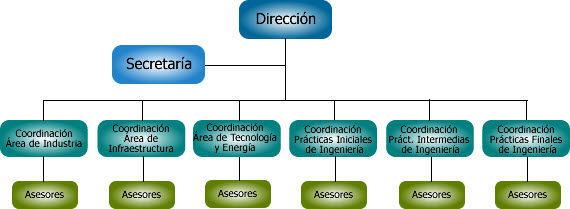
\includegraphics[width=1\linewidth]{images/201901-unidadeps-imagen01}
\figcaption{Organigrama Unidad de Prácticas de Ingeniería y EPS}

\end{minipage}

\end {flushleft}

\bigskip

\end {multicols}

\hypertarget{personal-administrativo-y-docente}{%
\section*{Personal Administrativo y Docente}\label{personal-administrativo-y-docente}}
\addcontentsline{toc}{section}{Personal Administrativo y Docente}

\begin{figure}[H]

{\centering 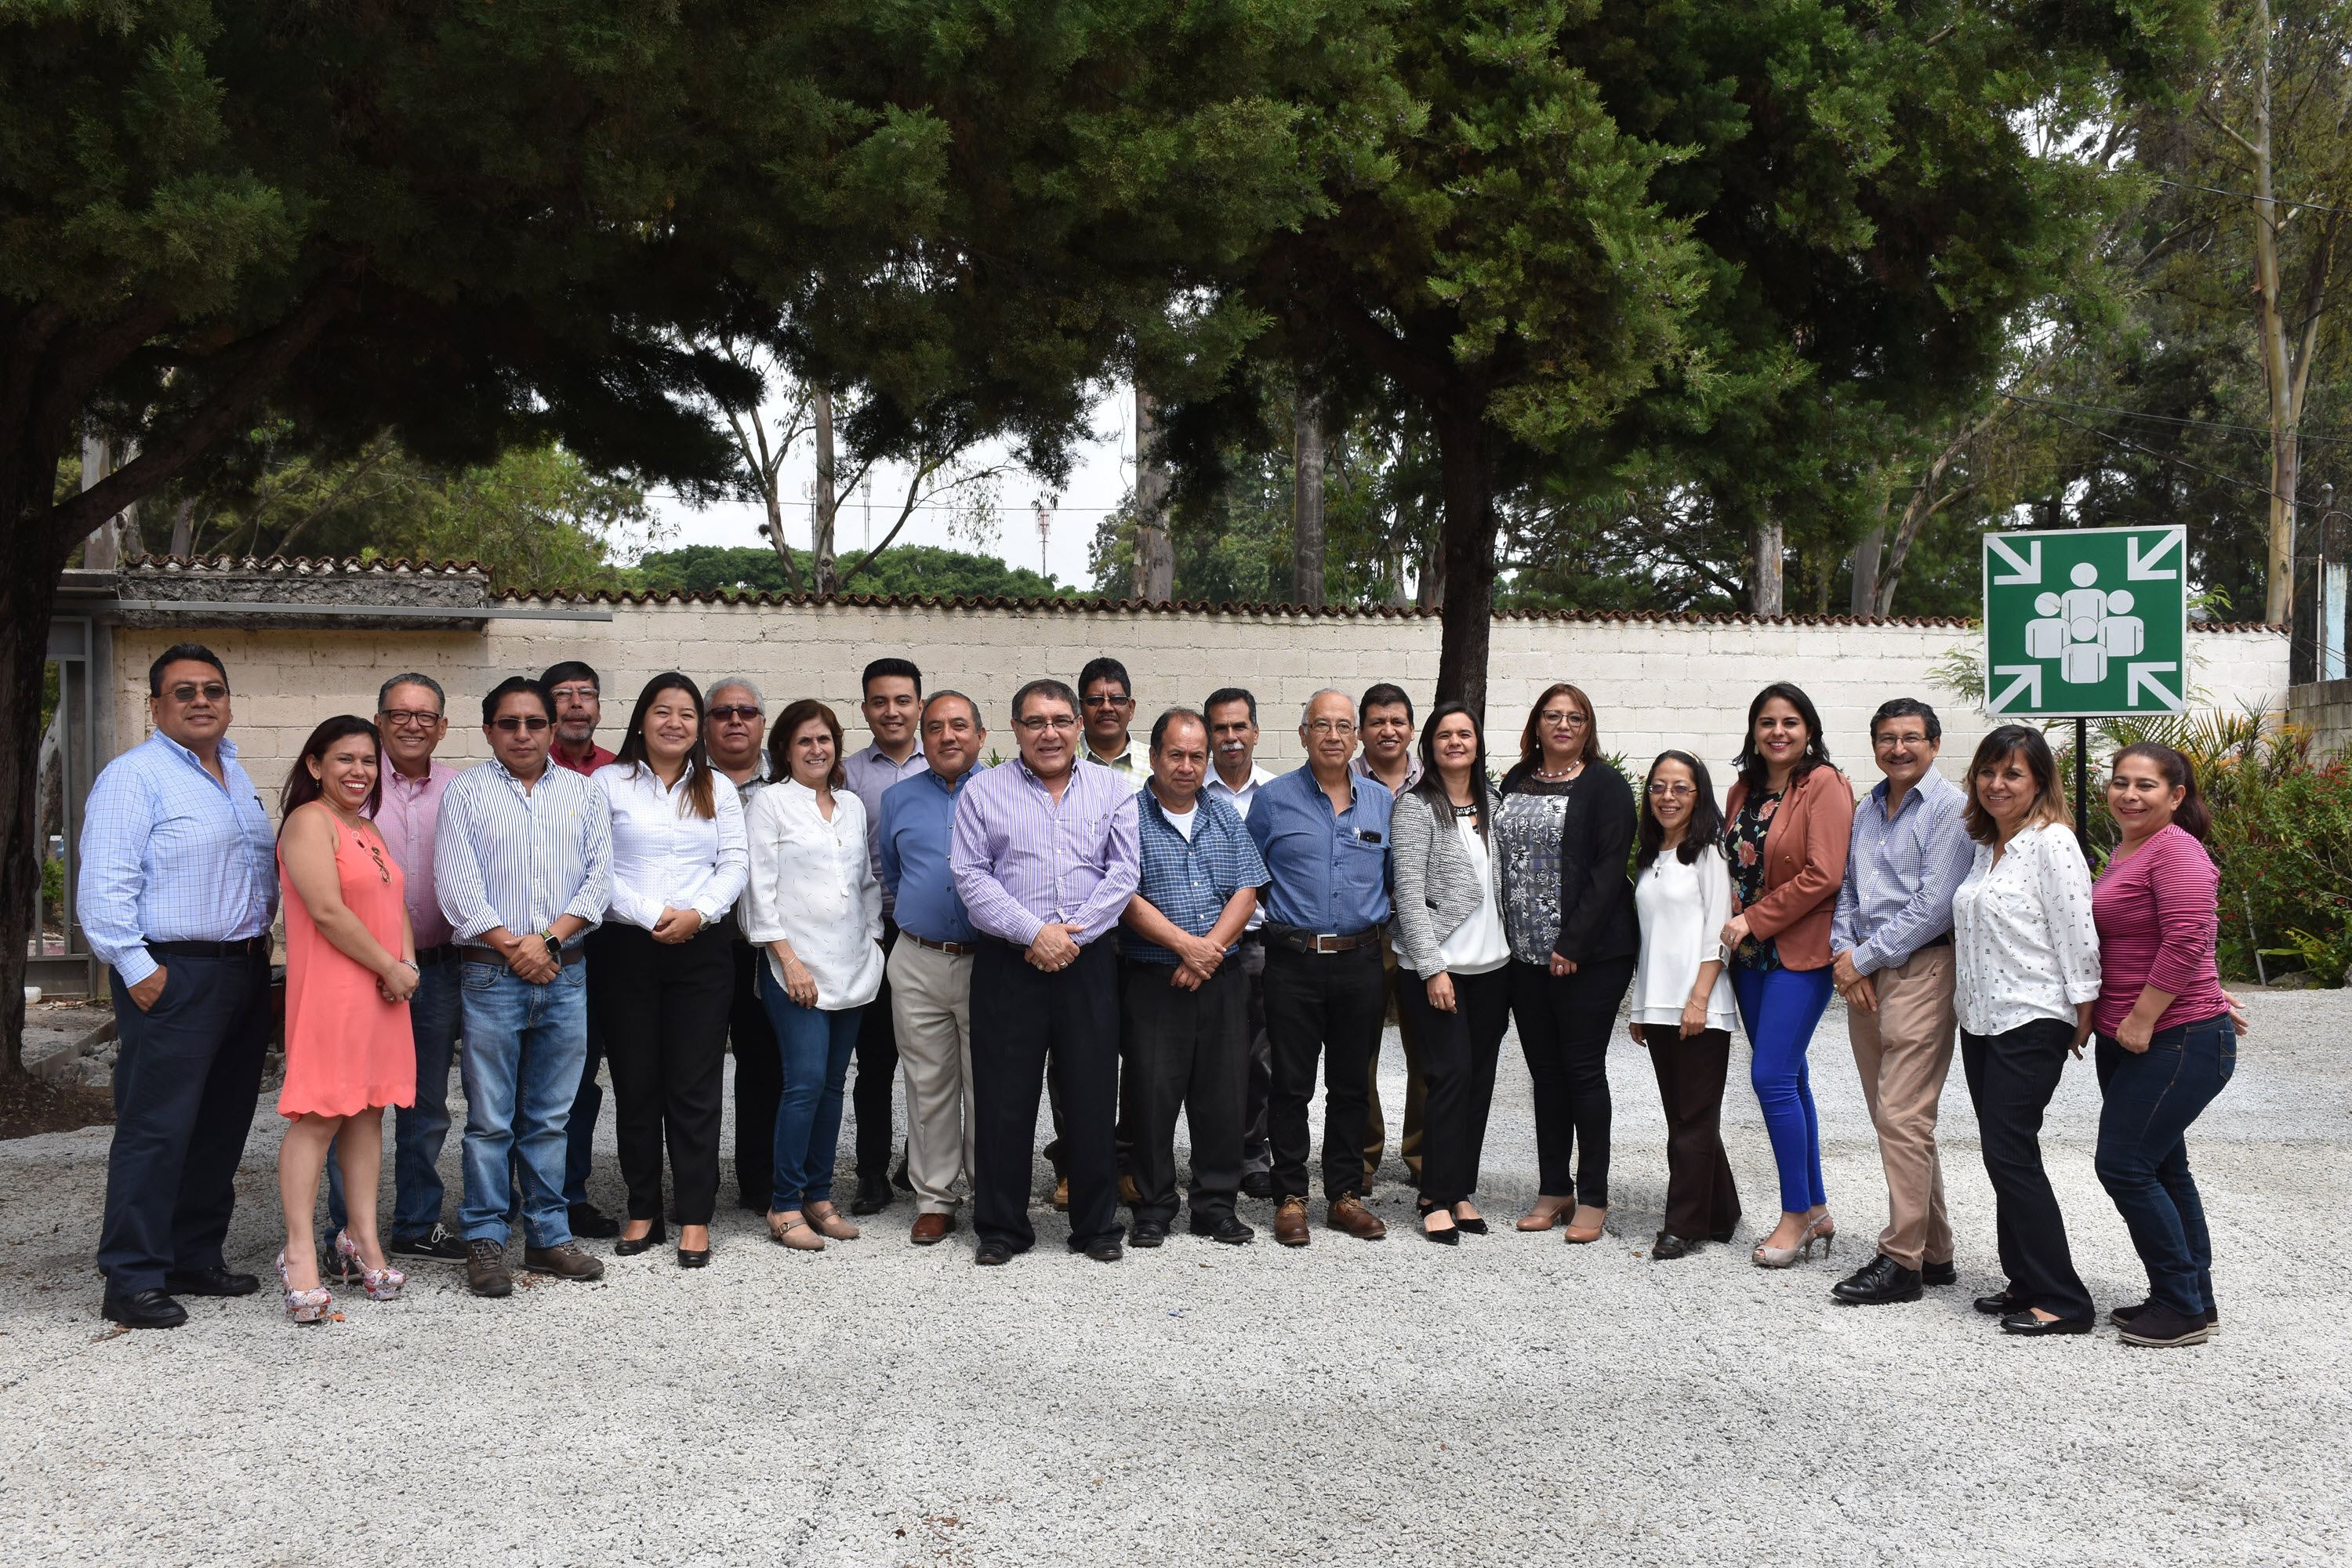
\includegraphics[width=0.78\linewidth]{images/201901-unidadeps-imagen02} 

}

\caption{Personal de Unidad de Prácticas de Ingeniería y Ejercicio Profesional Supervisado}\label{fig:unnamed-chunk-14}
\end{figure}

\hypertarget{descripcion-de-personal-administrativo-y-docente}{%
\section*{Descripción de Personal Administrativo y Docente}\label{descripcion-de-personal-administrativo-y-docente}}
\addcontentsline{toc}{section}{Descripción de Personal Administrativo y Docente}

\begin {multicols}{2}

A continuación nombres (Izquierda a Derecha):
\spacethreemilis

\begin{itemize}
\tightlist
\item
  Ingeniero Mecánico Emilio Vladimir Lux Monroy
  \spacetwomilis
\item
  Ingeniera Industrial Yocasta Ivanobla Ortíz del Cid
  \spacetwomilis
\item
  Ingeniero Civil Silvio José Rodríguez Serrano
  \spacetwomilis
\item
  Ingeniero Electricista Natanael Jonathan Requena Gómez
  \spacetwomilis
\item
  Ingeniero Mecánico Carlos Anibal Chicojay Coloma
  \spacetwomilis
\item
  Ingeniera Industrial Sindy Massiel Godinez Bautista
  \spacetwomilis
\item
  Ingeniero Civil Manuel Alfredo Arrivillaga Ochaeta
  \spacetwomilis
\item
  Ingeniera Civil Christa del Rosario Classon de Pinto
  \spacetwomilis
\item
  Ingeniero Mecánico Diego Israel Navarro Godinez
  \spacetwomilis
\item
  Ingeniero en Ciencias y Sistemas Sergio Leonel Gómez Bravo
  \spacetwomilis
\item
  Ingeniero Civil Oscar Argueta Hernández
  \spacetwomilis
\item
  Ingeniero Mecánico Edwin Estuardo Sarceño Zepeda
  \spacetwomilis
\item
  Ingeniero Civil Luis Gregorio Alfaro Véliz
  \spacetwomilis
\item
  Ingeniero Electricista Francisco Javier Gonzalez López
  \spacetwomilis
\item
  Ingeniero Civil Juan Merck Cos
  \spacetwomilis
\item
  Ingeniero Químico Sergio Alejandro Recinos
  \spacetwomilis
\item
  Ingeniera Industrial Sigrid Alitza Calderón de León
  \spacetwomilis
\item
  Ingeniera Industrial Norma Ileana Sarmiento Zeceña de Serrano
  \spacetwomilis
\item
  Ingeniera Química Lorena Victoria Pineda Cabrera
  \spacetwomilis
\item
  Ingeniera Industrial Rocio Carolina Medina Galindo
  \spacetwomilis
\item
  Ingeniero Industrial Jaime Humberto Batten Esquivel
  \spacetwomilis
\item
  Ingeniera Civil Mayra Rebeca García Soria de Sierra
  \spacetwomilis
\item
  Licenciada en Administración de Empresas Maria Roxana Alvarado Monterroso
\end{itemize}

\end {multicols}

\medskip

\HRule

\medskip

\hypertarget{mgarcia}{%
\chapter{Camino construido para las comunidades Matacuy, Concepción 2 y 3, Panzós, Alta Verapaz}\label{mgarcia}}

\begin {flushleft}

\tcolorboxcommand

\begin{minipage}[c]{3cm}

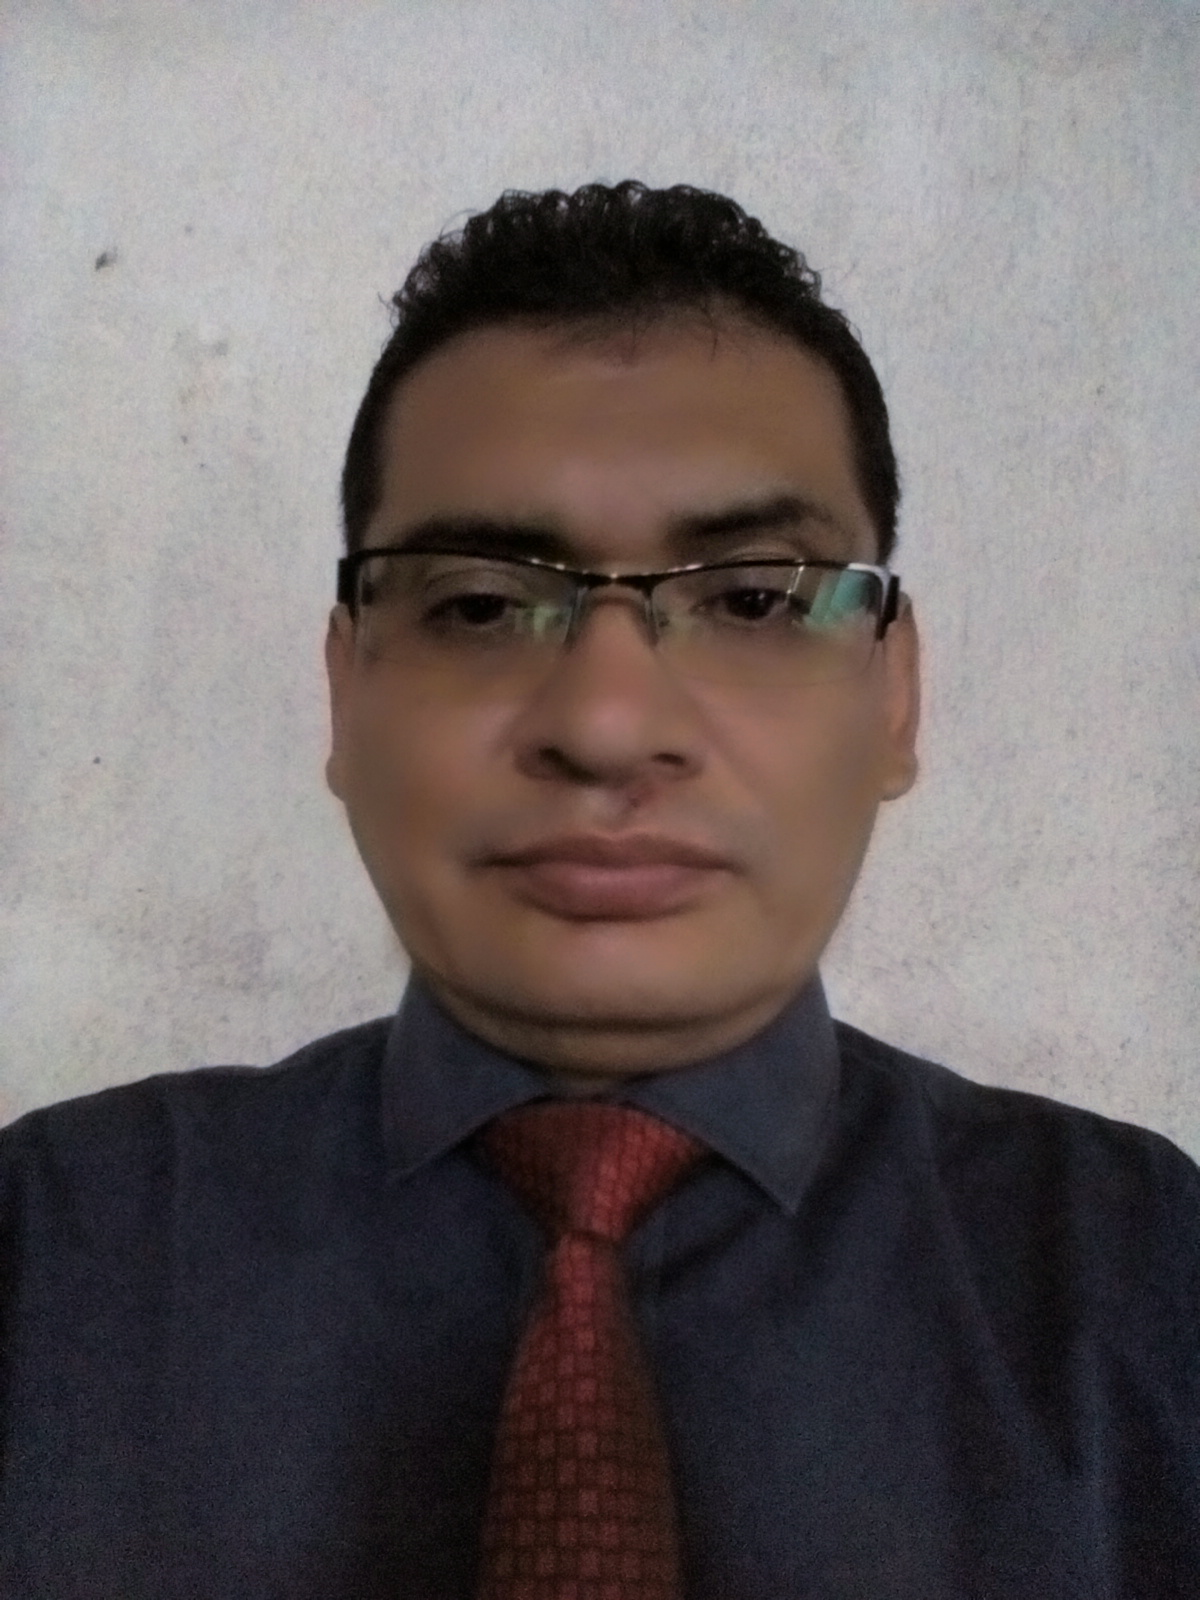
\includegraphics[width=2.5cm,height=\textheight]{images/image00_mgarcia.jpg}

\end{minipage}\begin{minipage}[c]{12cm}

\textbf{Autor:} \emph{Ing. Moisés Aarón García Chitay}\\
\textbf{Correo electrónico:} \emph{\href{mailto:gam1174100@gmail.com}{\nolinkurl{gam1174100@gmail.com}}}\\
\textbf{Fecha:} \emph{02 de mayo de 2019}

\end{minipage}

\end {tcolorbox}

\end {flushleft}

\hypertarget{palabras-clave}{%
\section*{Palabras Clave:}\label{palabras-clave}}
\addcontentsline{toc}{section}{Palabras Clave:}

\emph{Diseño, tramo carretero, Panzós.}

\begin {multicols*}{2}

\hypertarget{introduccion-1}{%
\section{Introducción}\label{introduccion-1}}

En el presente artículo se describe el proceso del proyecto realizado en el municipio de Panzós, Alta Verapaz. Este responde a las necesidades planteadas por la población de dicho municipio y que la Universidad de San Carlos, a través de la unidad de Ejercicio Profesional Supervisado, cumple con su proyección social para el desarrollo de las comunidades más lejanas, incentivando el progreso y desarrollo económico a través de obras de infraestructura planificadas por la municipalidad en mención.

A continuación, el informe proporcionado por la Municipalidad de Panzós, Alta Verapaz

\begin{figure}[H]

{\centering 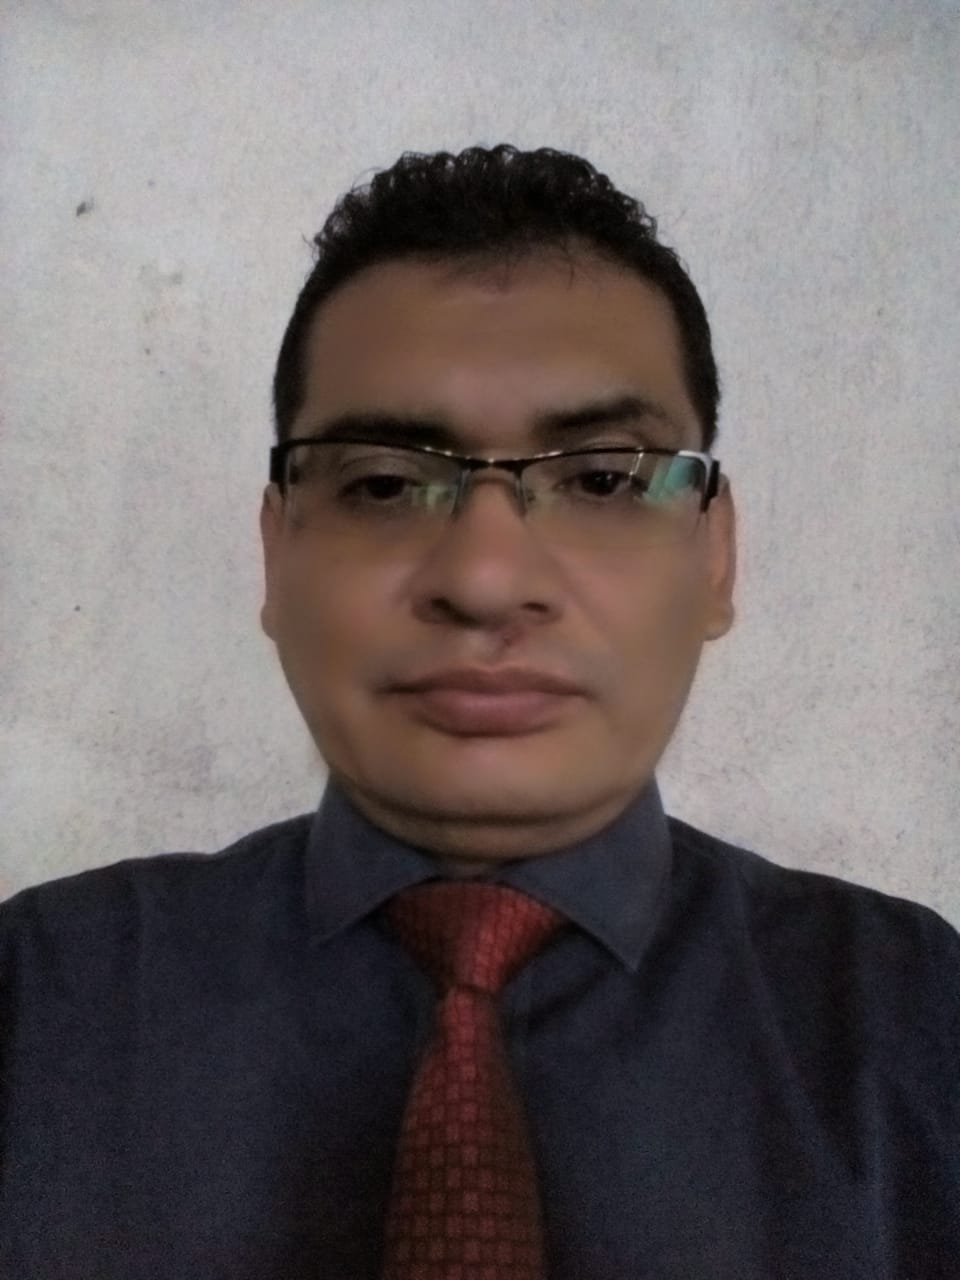
\includegraphics[width=0.14\linewidth]{images/image01_mgarcia} 

}

\caption{Municipalidad de Panzós, Alta Verapaz}\label{fig:unnamed-chunk-15}
\end{figure}

\spacetwominus
\spacetwominus
\spacetwominus

Administración 2,016 -- 2,020. Unidos por un Nuevo Panzós Sa'qach'ool La Municipalidad de Panzós realizó el mantenimiento y apertura de las carreteras de las comunidades Matacuy, de Concepción II y III, las cuales tienen las longitudes siguientes: de Matacuy a Concepción II, con un trabajo de 3700 metros y de Matacuy a Concepción III, con 3600 metros de distancia.

\hypertarget{articulo}{%
\section{Artículo}\label{articulo}}

\spacetwominus

Diseño del tramo carretero que comprende 4420 metros de longitud. Inicia en la aldea Matacuy, pasa por la aldea Tierra Linda y llega a la aldea San Antonio. Esta carretera será de beneficio para las comunidades mencionadas para lograr un crecimiento comercial y permitir un fácil acceso al lugar en cualquier época del año, además de un mejor traslado de sus productos agrícolas.

Se realizaron los estudios topográficos, toma de muestra de suelo, ensayos de laboratorio, planos, especificaciones y presupuesto del mismo.
Para este diseño, según las especificaciones de la Dirección General de Caminos para los diferentes tipos de carretera, se seleccionó una carretera tipo ``F''; ya que la topografía del lugar presenta características muy difíciles debido a que es una región montañosa. Se realizó el siguiente análisis del proyecto:

\spacetwominus
\spacetwominus

\hypertarget{caracteristicas-generales}{%
\subsection{Características generales:}\label{caracteristicas-generales}}

\spacetwominus

\begin{itemize}
\tightlist
\item
  Longitud del proyecto: 4+420 kilómetros
\item
  Tipo de carretera: rural basada en la típica ``F'' de la D.G.C.
\item
  Tipo de región: montañosa
\item
  Velocidad de diseño: 20 km/h
\item
  Tránsito promedio diario: no mayor de 100 vehículos
\item
  Ancho de terracería: 5,5 metros
\item
  Espesor de balasto: 0,20 metros
\item
  Pendiente máxima: 18 \%
\end{itemize}

\end {multicols*}

\begin{figure}[H]

{\centering 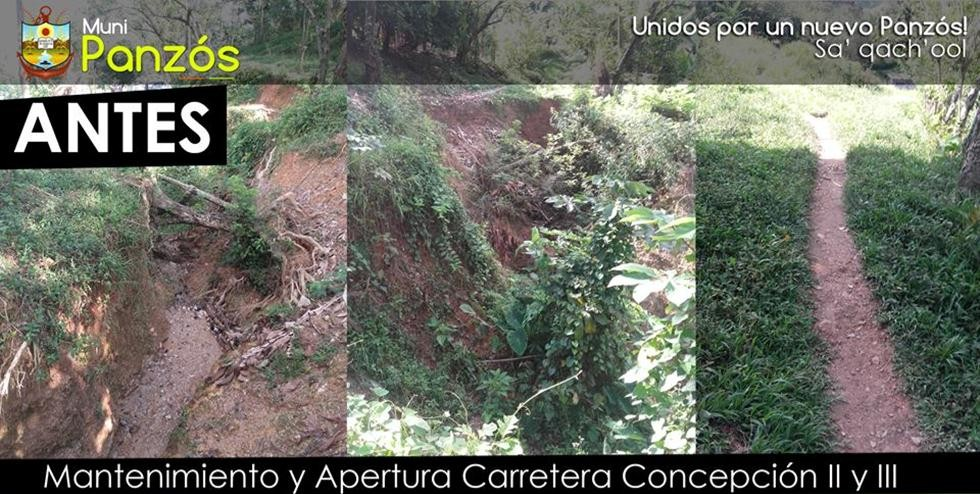
\includegraphics[width=0.8\linewidth]{images/image02_mgarcia} 

}

\caption{Carreteras Concepción II y III antes de iniciar los trabajos}\label{fig:unnamed-chunk-16}
\end{figure}

\begin{figure}[H]

{\centering 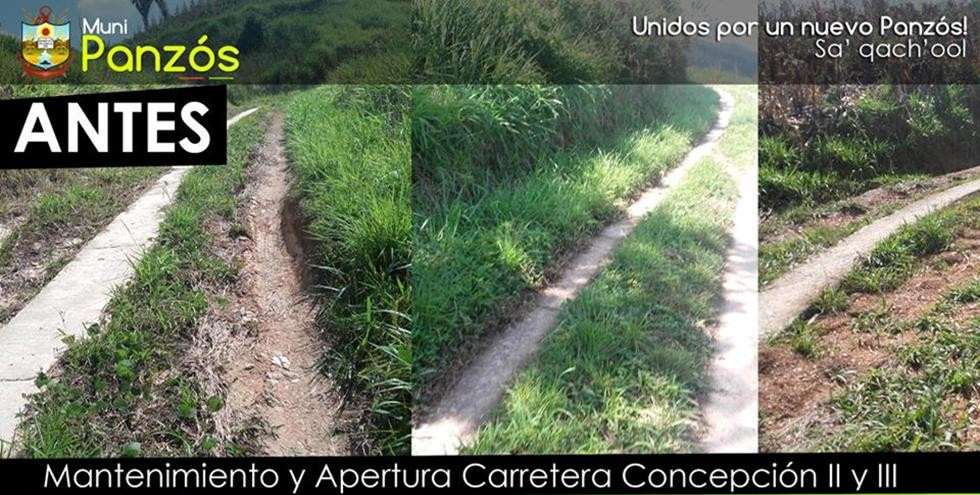
\includegraphics[width=0.8\linewidth]{images/image03_mgarcia} 

}

\caption{Carreteras Concepción II y III antes de iniciar los trabajos}\label{fig:unnamed-chunk-17}
\end{figure}

\begin {multicols}{2}

\spacetwomilis

Los trabajos necesarios para la preparación del terreno son: limpieza y desmonte del área del tramo, explotación de bancos de material, manejo y disposición final de los desechos sólidos provenientes de la limpieza, desmonte y cortes, excavación y nivelación, limpieza de derrame de lubricantes, combustibles u otros materiales provocados por la maquinaria.

\spacefourmilis

Sustancias o materiales que serán utilizados: diésel, aceites y lubricantes para la maquinaria y equipo que se va a utilizar; además, cemento, piedra, piedrín, arena y tubería de material corrugado.

Recursos naturales del área: el mismo material proveniente de los cortes, balasto proveniente de banco de materiales, estacas y trompos para referenciar los límites de la carretera.

\end {multicols}

\begin{figure}[H]

{\centering 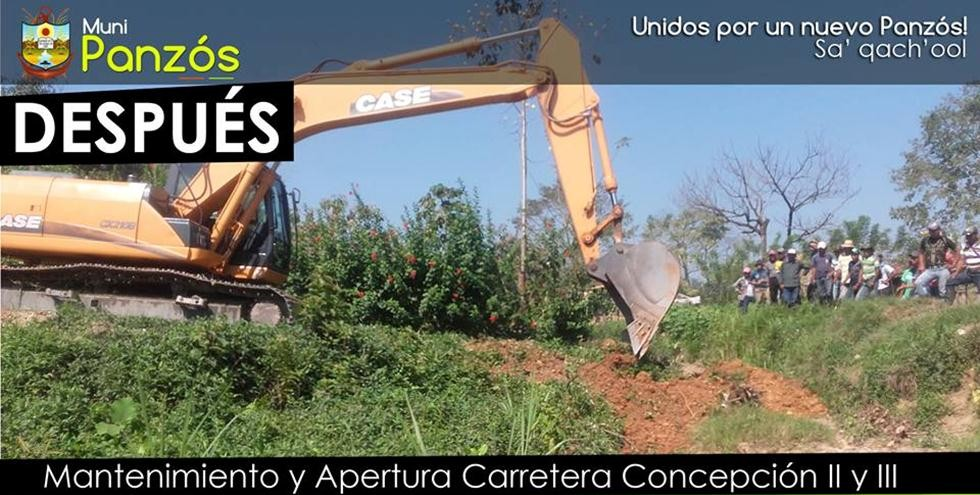
\includegraphics[width=0.7\linewidth]{images/image04_mgarcia} 

}

\caption{Inicio y proceso de mejoramiento de carretera}\label{fig:unnamed-chunk-18}
\end{figure}

\spacetwominus
\spacetwominus
\spacetwominus

\begin{figure}[H]

{\centering 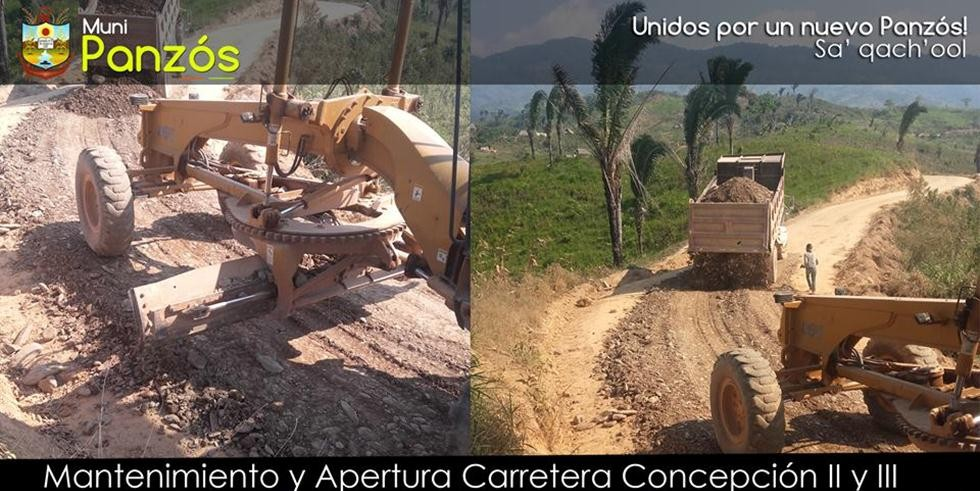
\includegraphics[width=0.7\linewidth]{images/image05_mgarcia} 

}

\caption{Inicio de trabajos de mantenimiento y mejoramiento de carretera Concepción II y III}\label{fig:unnamed-chunk-19}
\end{figure}

\begin {multicols}{2}

\spacetwominus
\spacetwominus

\hypertarget{impacto-ambiental-producido}{%
\subsection{Impacto ambiental producido}\label{impacto-ambiental-producido}}

\emph{Residuos o contaminantes que serán generados:} dentro de los residuos generados se tendrán las emisiones de partículas a la atmósfera, descarga de aguas residuales y lubricantes, entre otros.

\emph{Descarga de aguas residuales:} el manejo no correcto de excretas provenientes de los campamentos y otras áreas de trabajo puede generar contaminación del suelo y mantos de agua.

\emph{Desechos sólidos:} debido a la construcción y operación del proyecto se tendrán los residuos de material de excavación, así como desechos por el uso de maquinaria tales como: repuestos usados, filtros, neumáticos, entre otros; así como basura producida por los trabajadores.

\emph{Ruido o vibraciones:} por la utilización de maquinaria y equipo durante las fases de preparación del sitio, explotación de bancos de material y construcción de la carretera.

Para todos estos factores negativos debe existir un plan de contingencia, que disminuya su daño. Por ejemplo: en chapeo, destronque, excavación y nivelación de tierras, se propone poblar de vegetación en las áreas afectadas.

En el acarreo de materiales o específicamente de suelos, es necesario que en cada viaje que realice el camión de carga utilice una lona que evite desprendimiento de partículas al aire, ya que puede ser nocivo para la higiene del ser humano.

\end {multicols}

\begin {center}

\textbf{Finalización de mejoramiento de carretera}

\end {center}

\begin{figure}[H]

{\centering 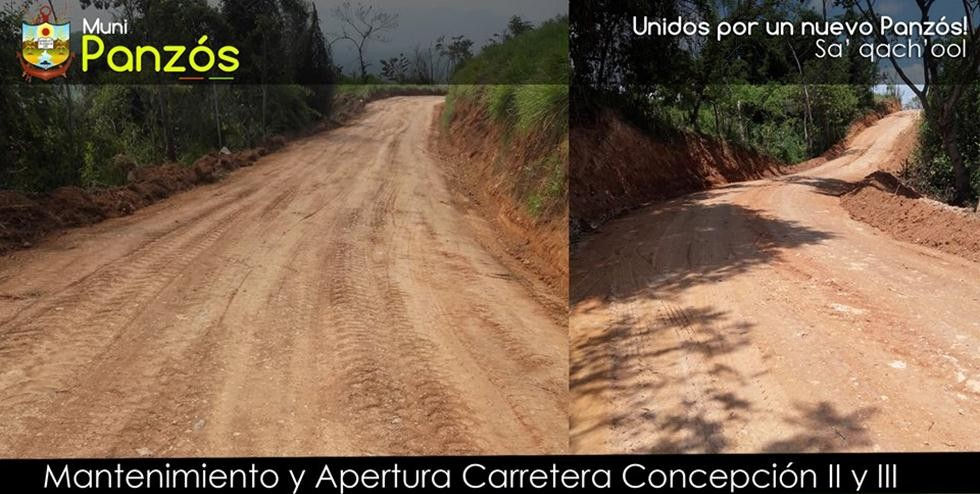
\includegraphics[width=0.7\linewidth]{images/image06_mgarcia} 

}

\caption{Trabajo finalizado de mejoramiento de carretera Concepción II y III}\label{fig:unnamed-chunk-20}
\end{figure}

\begin{figure}[H]

{\centering 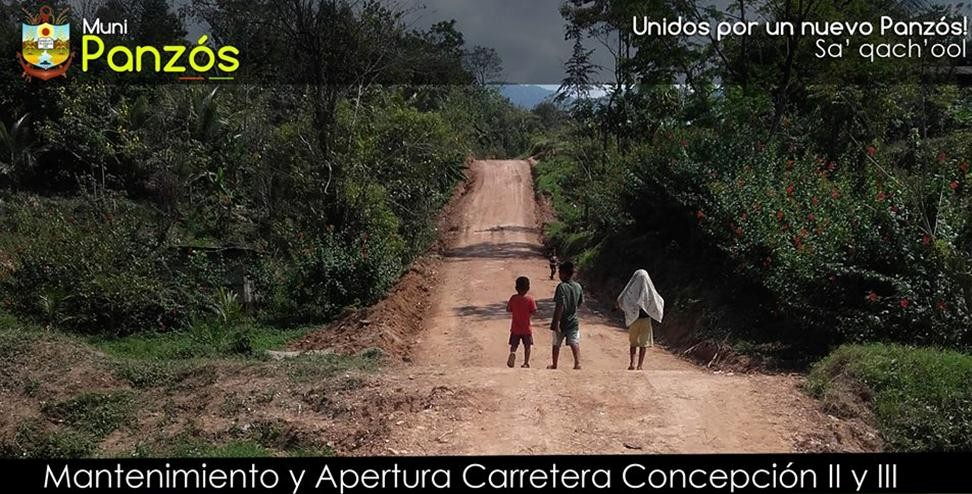
\includegraphics[width=0.7\linewidth]{images/image07_mgarcia} 

}

\caption{Trabajo finalizado de mejoramiento de carretera Concepción II y III}\label{fig:unnamed-chunk-21}
\end{figure}

\begin {multicols}{2}

\spacethreemilis

\hypertarget{conclusiones}{%
\section{Conclusiones}\label{conclusiones}}

\begin{itemize}
\item
  El tramo carretero hacia la aldea San Antonio será de mucho beneficio para los habitantes, ya que podrán trasladarse con mayor facilidad y rapidez hacia el lugar donde tienen sus cultivos, además podrán vender sus productos de forma directa y obtener beneficios económicos para las familias. La carretera está diseñada según las especificaciones de la Dirección General de Caminos para un período de 20 años.
\item
  El Ejercicio Profesional Supervisado permitió que el estudiante desarrollara sus conocimientos teórico-prácticos, de tal forma, que se logró un beneficio para las comunidades por medio de proyectos de infraestructura, así como una perspectiva real acerca de las necesidades que tiene el país.
\item
  Con la elaboración del proyecto se cumplió con la misión social de la Universidad de San Carlos de Guatemala y la Facultad de Ingeniería, ya que ninguna de estas comunidades cuenta con los fondos necesarios para financiar estos proyectos.
\end{itemize}

\hypertarget{referencias}{%
\section{Referencias}\label{referencias}}

\begin{itemize}
\tightlist
\item
  {[}1{]} \href{http://www.repositorio.usac.edu.gt/4300/}{García, M.} (25 de abril 2016). \href{https://www.usac.edu.gt/}{USAC:} \href{http://www.repositorio.usac.edu.gt/4300/}{\emph{Diseño del sistema de abastecimiento de agua potable para la aldea Tierra Linda y de la carretera hacia la aldea San Antonio, municipio de Panzós, Alta Verapaz}}. Recuperado de: \url{https://bit.ly/3gD6BfX}. {[}Último acceso: mayo de 2020{]}.
\end{itemize}

\end {multicols}

\medskip

\HRule

\medskip

\hypertarget{jgarcia}{%
\chapter{EPS, expectativa y desarrollo}\label{jgarcia}}

\begin {flushleft}

\tcolorboxcommand

\begin{minipage}[c]{3cm}

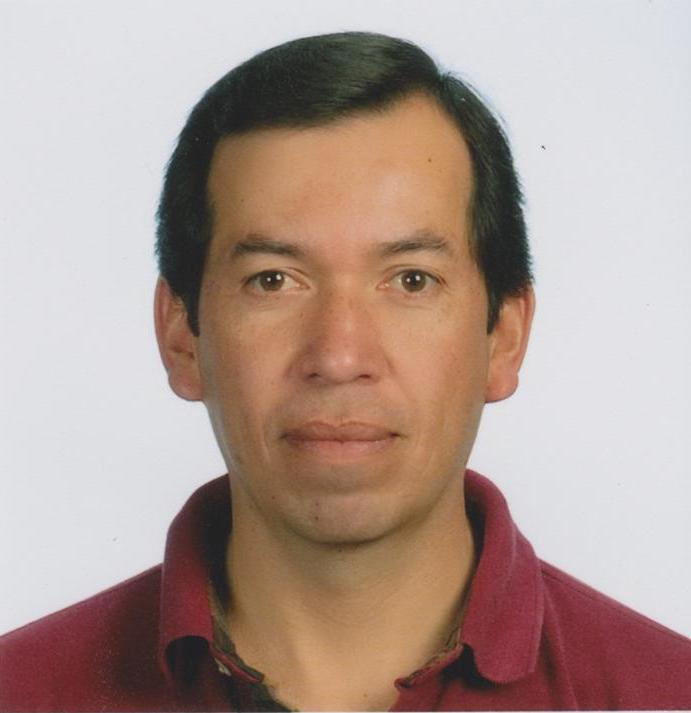
\includegraphics[width=2.5cm,height=\textheight]{images/image01_jgarcia.jpg}

\end{minipage}\begin{minipage}[c]{12cm}

\textbf{Autor:} \emph{Ing. Jaime Manuel García Baldizón}\\
\textbf{Correo electrónico:} \emph{\href{mailto:jgarciab23@gmail.com}{\nolinkurl{jgarciab23@gmail.com}}}\\
\textbf{Fecha:} \emph{02 de mayo de 2019}

\end{minipage}

\end {tcolorbox}

\end {flushleft}

\begin {multicols}{2}

\hypertarget{eps-expectativa-y-desarrollo}{%
\section{EPS, expectativa y desarrollo}\label{eps-expectativa-y-desarrollo}}

Concluir el pénsum de Ingeniería Civil fue por demás una gran experiencia, lograr vencer todas las barreras, todos los desafíos impuestos por los catedráticos, lograr cerrar cada área de estudios que parecía ser imposible; y para festejarlo nos lanzamos al tan ansiado ``piletazo de ingeniería'', luego de los abrazos, felicitaciones y admiración de todos nuestros familiares y amigos, iniciamos el camino final hacia el Francisco Vela.

Elegí la opción EPS de 6 meses, porque me interesaba convivir directamente con las comunidades rurales y devolver, de alguna forma y mínimamente, la inversión realizada por la sociedad a través de la Universidad de San Carlos. Luego de presentar toda mi documentación fui aceptado para el desarrollo del EPS. Desde un principio mi asesor impulsó ánimo en el grupo y se empeñó por demostrar que éramos capaces de terminarlo en el tiempo asignado; que si en alguna área de estudio estábamos débiles, no importaba, ahora podíamos mejorar y complementar nuestros estudios.

No lograba comprender por qué desde un principio nuestro asesor se preocupaba por la posibilidad de no concluir el EPS, si tenía la capacidad y los estudios necesarios; además, significaba la meta final, la prioridad total y sin tener que asistir a las aulas, podía dedicarme el 100\% al proyecto asignado.

Durante la investigación y presentación de proyectos para la aprobación por parte de la Dirección de EPS, fue posible conocer las necesidades de la comunidad, lograr la comunicación con los líderes comunales y comprender que falta desarrollar gran cantidad de infraestructura básica necesaria para garantizar salud, educación y desarrollo en el área rural.

Todo avanzaba bien y el tiempo para realizar esta parte concluyente de la carrera era el adecuado; cuando concluí el protocolo de desarrollo del trabajo profesional, empecé a investigar sobre documentos necesarios que no sabía dónde localizar; inició la primera recolección de firmas y la búsqueda de opinión de los catedráticos cuando no siempre aceptaban cualquier proyecto desde el primer intento y requerían que se investigara más; pero sin decirnos sobre qué, también pedían que abundáramos más sobre temas especializados no vistos en clase o que fueron percibidos de forma muy somera. Fue necesario visitarlos varias veces y pedir que se tomaran el tiempo para analizar los proyectos, hasta que por fin mi protocolo fue aprobado.

Inicié el proyecto formalmente, solicité equipo para realizar las medidas topográficas necesarias, estudios de suelos, entre otros, y solicitar el apoyo de las organizaciones comunales para llevar a cabo los estudios iniciales y el censo comunal. Con toda la información de campo recabada procedí a la creación y diseño de la obra que, a mi criterio, solucionaba el problema planteado.

En este punto inició mi temor, el comprender que estudiamos cursos solo para aprobar exámenes, que lo aprendido en clases no era suficiente para solucionar dudas, porque las obras que se tenían que desarrollar eran, por mucho, mayores y más complejas que las vistas en clase. No era posible ir a preguntar, porque cómo es posible que un estudiante que ya cerró pénsum esté preguntando aspectos básicos, y cuando me animaba a preguntar sobre algún tema muchas veces la respuesta fue: ``eso lo debió haber visto en clase, ¿no se acuerda?''. Inició mi disertación enfatizando en que: ``somos capaces de realizar este estudio'', el plan de acción que me propuse no abarca todos los temas necesarios, es posible que no tenga la capacidad de diseñar esta obra. Momentos muy difíciles que representaron el continuar o simplemente abandonar el EPS.

Fue solo el deseo de culminar y cumplir con el anhelo de llegar a ser un Ingeniero, que me hizo pedir ayuda; reconocer que no sabía el camino a seguir, que debía estudiar mucho para realizar las obras propuestas. Es aquí donde las recomendaciones iniciales de nuestro asesor tomaron fuerza, expresé a mi asesor mis dudas y temores; acepté mis deficiencias teóricas y el no saber cómo trazar un plan de acción específico, que sentía demasiada presión y no tenía la capacidad de lograrlo. Mi pensamiento era que me regresaría a estudiar todos los cursos nuevamente, pero necesitaba expresarlo y solicitar ayuda.

Sin embargo, mi asesor muy tranquilamente me indicó que era normal el temor, que todas las dudas e incapacidad que sentía eran parte del proceso de aprendizaje; que él podía ayudarme, pero para ello tenía que pedir y estar dispuesto a aceptar la ayuda. Debía entender que podía guiarme hacia la meta final, pero tenía que trabajar duro, estudiar mucho y comprometerme con la ruta por la cual debía transitar.

Fueron meses de trabajo duro y estudio constante; de investigar, consultar y entender muchos temas que fueron tratados en clase, pero sin la debida atención al respecto; sin embargo, el éxito no se hizo esperar. El día tan esperado finalmente llegó, y en una sesión de trabajo mi asesor dijo: ``lo lograste, es hora de solicitar tu examen general privado''.

Es una satisfacción personal única, confrontar mis temores, aprender y reforzar todas las áreas de estudio aplicadas a un proyecto, entender que la universidad es una base fundamental, pero que debemos estar en constante capacitación y aprendizaje; por sobre todo, un aspecto muy importante fue la vivencia significante de apoyar a las comunidades tan necesitadas en nuestro país, compartir con ellos directamente y ser partícipe de una solución; recibir el reconocimiento y agradecimiento de la comunidad es sentir que valió la pena todo el esfuerzo; solo a través de esta experiencia pude aprender y entender el Ejercicio Profesional Supervisado.

Expreso mi agradecimiento a la Unidad de EPS por su solidaridad e interés en guiar a cada estudiante hacia la solución de sus proyectos; su esfuerzo por impulsar y animar en todo el proceso y en especial agradecer a mi asesor Ing. Juan Merck por su tiempo, respaldo y excelente guía. Solo me toca esperar que algún día logre ver edificada la obra proyectada y que la comunidad se beneficie a partir del estudio entregado.

\end {multicols}

\medskip

\HRule

\medskip

\hypertarget{bflorian1}{%
\chapter{Portal para la transmisión del canal TEVE Humanidades en vivo de forma simultánea}\label{bflorian1}}

\begin {flushleft}

\tcolorboxcommand

\begin{minipage}[c]{3cm}

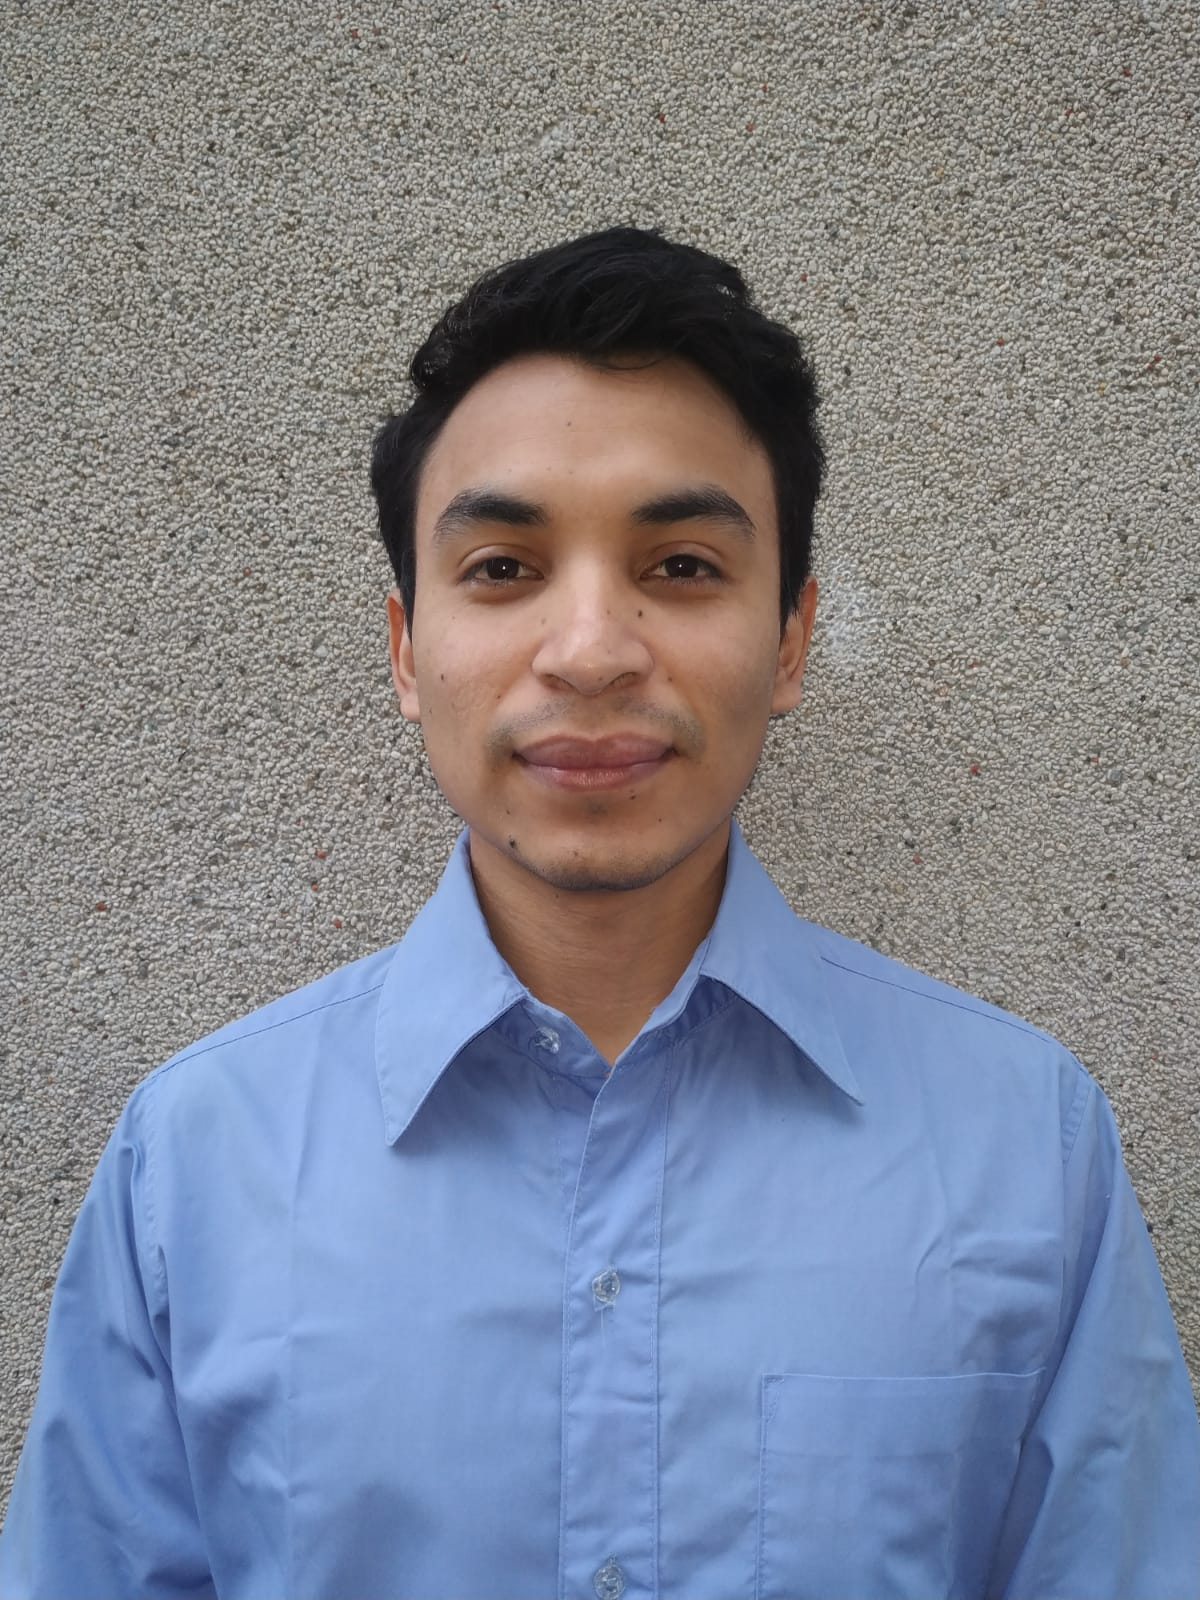
\includegraphics[width=2.5cm,height=\textheight]{images/image01_bflorian1.jpg}

\end{minipage}\begin{minipage}[c]{12cm}

\textbf{Autor:} \emph{Braian Staimer Florián Montenegro}\\
\textbf{Correo electrónico:} \emph{\href{mailto:braianflorian@gmail.com}{\nolinkurl{braianflorian@gmail.com}}}\\
\textbf{Fecha:} \emph{20 de octubre de 2019}

\end{minipage}

\end {tcolorbox}

\end {flushleft}

\hypertarget{resumen}{%
\section*{Resumen}\label{resumen}}
\addcontentsline{toc}{section}{Resumen}

La Facultad de Humanidades de la Universidad de San Carlos de Guatemala busca que el público general pueda recibir la transmisión para ver videos en vivo y en diferido del contenido del canal TEVE Humanidades. El proceso anterior estaba limitado a transmitir en una única plataforma desde una misma señal de video. No se tenía una plataforma propia que cumpliera con los lineamientos para la transmisión en cable nacional y mundial. El proyecto cumplió con las expectativas de quienes lo propusieron, desarrollaron e implementaron.

\hypertarget{abstract}{%
\section*{Abstract}\label{abstract}}
\addcontentsline{toc}{section}{Abstract}

The Faculty of Humanities of the Universidad de San Carlos de Guatemala seeks that the general public can receive the transmission to watch live and deferred videos of the content of the TEVE Humanidades channel. The previous process was limited to transmitting on a single platform from the same video signal. There was no platform of its own that met the guidelines for cable transmission nationwide and worldwide. The project met the expectations of those who proposed the project and those who developed and implemented it.

\hypertarget{palabras-clave-1}{%
\section*{Palabras Clave:}\label{palabras-clave-1}}
\addcontentsline{toc}{section}{Palabras Clave:}

\emph{EPS, plataformas de transmisión de video, servidor de video.}

\begin {multicols}{2}

\hypertarget{introduccion-2}{%
\section{Introducción}\label{introduccion-2}}

La Facultad de Humanidades de la Universidad de San Carlos de Guatemala cuenta con el canal de TEVE Humanidades, creada para transmitir eventos relacionados con la facultad; tal es el caso de la graduación de sus estudiantes, celebración de eventos culturales, entre otros más. TEVE Humanidades no tenía una plataforma para la transmisión de video en vivo; por lo que hacían uso de servicios de terceros. No se podía transmitir en más de una plataforma al mismo tiempo desde una misma señal de video; no existían lineamientos tecnológicos para la trasmisión en cable nacional y mundial. Debido a lo anterior, surgió la necesidad de desarrollar un portal web y configurar un servidor de transmisión de video en vivo para el canal de TEVE Humanidades que transmita video en vivo desde una misma señal, hacia múltiples plataformas, incluyendo el portal antes mencionado.

\hypertarget{articulo-1}{%
\section{Artículo}\label{articulo-1}}

\hypertarget{el-problema}{%
\subsection{El problema}\label{el-problema}}

Antes de la implementación del proyecto TEVE Humanidades, con sede en la Facultad de Humanidades de la Universidad de San Carlos de Guatemala, no se contaba con una plataforma para la transmisión de video en vivo; por lo que hacían uso de servicios de terceros. Únicamente se podía transmitir en una plataforma al mismo tiempo desde una señal de video; no se tenía un sistema de almacenamiento de videos que permitiera al público general sintonizar los videos en diferido, tampoco existían lineamientos tecnológicos para la trasmisión en cable nacional y mundial.

\spacethreemilis

\hypertarget{el-flujo-de-transmision-de-video-en-vivo-es-el-siguiente}{%
\subsection{El flujo de transmisión de video en vivo es el siguiente:}\label{el-flujo-de-transmision-de-video-en-vivo-es-el-siguiente}}

\begin{itemize}
\tightlist
\item
  El equipo de grabación realiza los preparativos para ejecutar la grabación de video y transmisión en vivo.
\end{itemize}

\spacetwomilis

\begin{itemize}
\tightlist
\item
  El equipo de grabación verifica que todo esté funcionando correctamente.
\end{itemize}

\spacetwomilis

\begin{itemize}
\tightlist
\item
  Una vez el entorno de grabación esté listo, un operador de cámara realiza la captura de video del evento que se desee transmitir en vivo; la señal de video proveniente de las cámaras es convertida de HDMI a SDI, por medio de un dispositivo externo, con el objetivo de permitir la compatibilidad entre dispositivos; luego la señal es recibida por el mezclador por medio de las entradas SDI, las cuales permiten resincronizar las señales y convertir el formato para adaptarlo al del mezclador.
\end{itemize}

\spacetwomilis

\begin{itemize}
\item
  Un director de cámara selecciona la vista de cámara que mejor convenga en cada momento para la transmisión de video; la señal elegida es enviada a una plataforma portátil de grabación.
\item
  De acuerdo con el evento que se esté transmi-
  tiendo, un operador puede grabarlo en tarjetas SD, para su posterior utilización.
\end{itemize}

\spacetwomilis

\begin{itemize}
\tightlist
\item
  Un operador ingresa a la plataforma de terceros, en donde se realizará la transmisión, y obtiene una dirección hacían donde se hará la emisión de video.
\end{itemize}

\spacetwomilis

\begin{itemize}
\tightlist
\item
  Otro operador hace uso de un programa para la emisión de video por medio del enlace obtenido.
\end{itemize}

\spacetwomilis

\begin{itemize}
\tightlist
\item
  Un operador realiza las configuraciones necesarias en un programa para la emisión de video; actualmente se utiliza el programa OBS.
\end{itemize}

\spacetwomilis

\begin{itemize}
\tightlist
\item
  Un operador inicia la transmisión de video en vivo a través de la plataforma establecida.
\end{itemize}

\spacethreemilis

\hypertarget{solucion-planteada}{%
\subsection{Solución planteada}\label{solucion-planteada}}

Con base en las necesidades planteadas se establecieron los siguientes objetivos para el proyecto:

\begin{itemize}
\tightlist
\item
  Desarrollar un gestor de videos para que el público general lo pueda ver en diferido a través del portal.
\item
  Establecer los lineamientos tecnológicos necesarios para transmitir en cable nacional.
\item
  Programar un servidor para transmitir video en vivo.
\end{itemize}

\spacethreemilis

\hypertarget{desarrollo-e-implementacion-del-proyecto}{%
\subsection{Desarrollo e implementación del proyecto}\label{desarrollo-e-implementacion-del-proyecto}}

Se desarrolló un portal web dinámico donde el público general puede recibir la transmisión para ver videos en vivo y en diferido. Se realizó la interface donde el administrador decida a qué otras plataformas, se transmitirá de forma simultánea. Se provee un gestor de videos para almacenamiento de archivos en formato de video de forma manual o automática. Además, permite agregar publicaciones multimedia en una sección específica. Se desarrolló un servidor para transmitir video en vivo, que lanza la señal de video a diferentes plataformas, tanto propias como de terceros. Se cuenta con un módulo de almacenamiento de videos, con opción de guardar el video que se esté transmitiendo, o contenido subido de forma manual. Así también, un módulo de codificación de video que permite la retransmisión de la señal de video en diferentes calidades. Además, se definieron los lineamientos necesarios para la transmisión en cable nacional.

\hypertarget{proyecto-implementado}{%
\subsection{Proyecto implementado}\label{proyecto-implementado}}

Una vez implementado el proyecto, el flujo del proceso cambió de la siguiente manera:

\end {multicols}

\begin {flushleft}
\noindent\begin{minipage}[c]{\columnwidth}

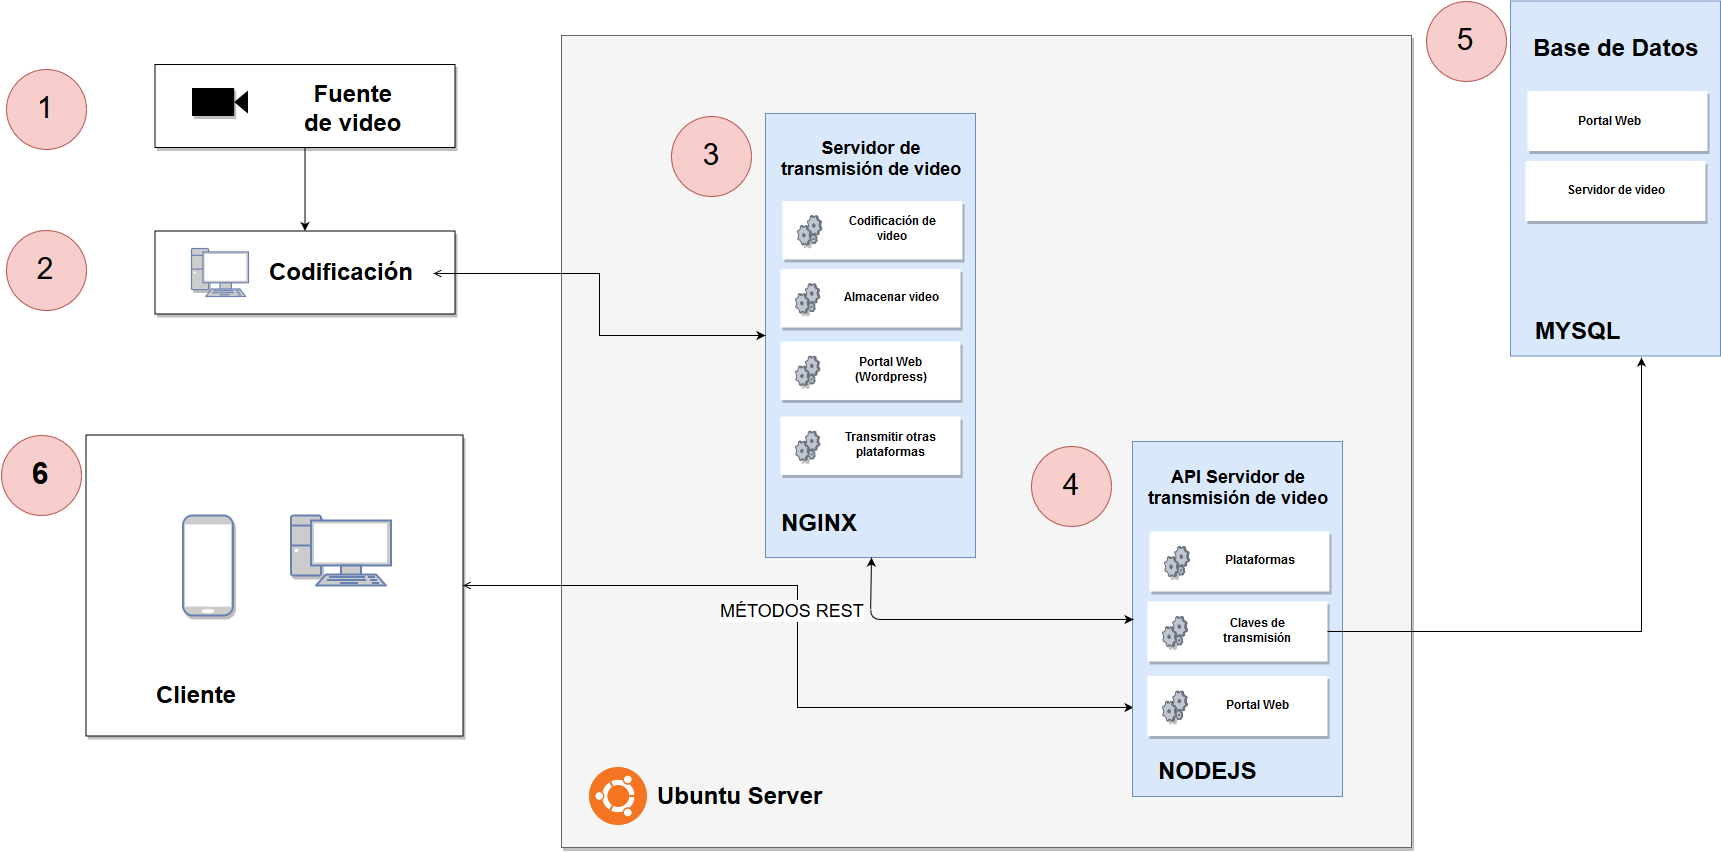
\includegraphics[width=1\linewidth]{images/image02_bflorian1}
\figcaption{Vista física de la aplicación. Fuente: Elaboración propia}

\end{minipage}

\end {flushleft}

\begin {multicols}{2}

\spacesixmilis
\spacesixmilis

\hypertarget{el-flujo-que-se-muestra-en-la-figura-se-describe-a-continuacion}{%
\subsection{El flujo que se muestra en la figura se describe a continuación:}\label{el-flujo-que-se-muestra-en-la-figura-se-describe-a-continuacion}}

\spacetwomilis

• El equipo de grabación realiza los preparativos para efectuar la grabación de video y transmisión en vivo. Una vez el entorno de grabación esté listo, un operador de cámara realiza la captura de video del evento que se desee transmitir en vivo.

• Un operador realiza las configuraciones necesarias en un programa para la emisión de video; actualmente se utiliza el programa OBS. Un operador inicia la transmisión de video en vivo a través de la plataforma establecida.

• El servidor de transmisión codifica la señal de video entrante y la transmite hacia las diferentes plataformas previamente configuradas.

• La interface entre el portal web y el servidor de transmisión de video permite por medio del protocolo de intercambio y manipulación de datos REST, configurar los parámetros para la transmisión de video en vivo.

• Se hace uso de una base de datos relacional para almacenar la información utilizada en el portal web y en el servidor de transmisión de video en vivo.

\spacesixmilis

• El público general, a través del portal web, puede sintonizar la transmisión de video en vivo, videos en diferido y publicaciones de multimedios.

\spacethreemilis

\hypertarget{lineamientos-tecnologicos-necesarios-para-transmitir-en-cable-nacional}{%
\subsection{Lineamientos tecnológicos necesarios para transmitir en cable nacional}\label{lineamientos-tecnologicos-necesarios-para-transmitir-en-cable-nacional}}

\spacethreemilis

Llevar la señal de TEVE HUMANIDADES a la empresa de cable sería por demás interesante, porque su alcance aumentaría exponencialmente a 2 millones de personas en todo el país, aproximadamente. Sin embargo, hay condiciones que las empresas de cable establecen para agregar a su guía de programación un canal de televisión nuevo; entre ellas pueden citarse:

• Una señal nítida, la cual se puede generar en TEVE HUMANIDADES, con la compra de un ancho de banda de internet de 8 megas, con servicio dedicado.

• Una programación interesante, amena y profesional. Para lo cual se necesitan dos productores y dos presentadores en TEVE HUMANIDADES.

• Una programación continua. Solo se logrará con el personal mínimo necesario arriba indicado, y con la colaboración de pedagogos y productores de la Facultad de Humanidades.

\hypertarget{conclusiones-1}{%
\section{Conclusiones}\label{conclusiones-1}}

• Se desarrolló un gestor de videos que permite que el público general, a través del portal web, pueda sintonizar la transmisión de video en vivo, videos en diferido y publicaciones de multimedios.

• Se crearon los lineamientos tecnológicos necesa-
rios para transmitir en cable nacional.

• Se programó un servidor para transmitir video en vivo hacia múltiples plataformas.

\hypertarget{recomendaciones}{%
\section{Recomendaciones}\label{recomendaciones}}

• Realizar auditorías periódicas al sistema para buscar y corregir posibles vulnerabilidades de seguridad.

• Revisar periódicamente si hay cambios en los estándares para transmitir en cable nacional.

• Capacitar al personal para el uso correcto del sistema, con el fin de evitar errores en la configuración del mismo. De la misma manera, llevar un control estadístico de consumo de recursos, para pronosticar cuándo el sistema se verá afectado por falta de recursos debido al crecimiento del mismo.

\hypertarget{referencias-1}{%
\section{Referencias}\label{referencias-1}}

\begin{itemize}
\tightlist
\item
  {[}1{]} \href{http://humanidades.usac.edu.gt/portal/}{Facultad de Humanidades, USAC}. \href{http://humanidades.usac.edu.gt}{USAC:} \href{http://humanidades.usac.edu.gt/portal/}{\emph{Facultad de Humanidades, USAC}}. Recuperado de: \url{http://humanidades.usac.edu.gt/portal/}. {[}Último acceso: octubre 2016{]}.
\end{itemize}

\end {multicols}

\medskip

\HRule

\medskip

\hypertarget{rherrera}{%
\chapter{Automatización de procesos con tecnologías de la información}\label{rherrera}}

\begin {flushleft}

\tcolorboxcommand

\begin{minipage}[c]{3cm}

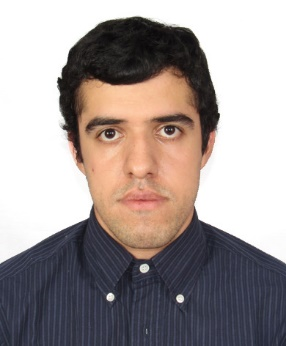
\includegraphics[width=2.5cm,height=\textheight]{images/image01_rherrera.jpg}

\end{minipage}\begin{minipage}[c]{12cm}

\textbf{Autor:} \emph{Ing. Rodrigo Antonio Herrera de León}\\
\textbf{Correo electrónico:} \emph{\href{mailto:herrerarodrigo750@gmail.com}{\nolinkurl{herrerarodrigo750@gmail.com}}}\\
\textbf{Fecha:} \emph{02 de noviembre de 2019}

\end{minipage}

\end {tcolorbox}

\end {flushleft}

\hypertarget{resumen-1}{%
\section*{Resumen}\label{resumen-1}}
\addcontentsline{toc}{section}{Resumen}

El presente trabajo describe el proyecto ejecutado en la Facultad de Humanidades para automatizar el proceso que los estudiantes siguen cuando se asignan y pagan por exámenes de recuperación. El proyecto también optimizó el ingreso de las notas de dichos exámenes y se desarrolló un sistema para llevar registro de las confirmaciones de pago. Estos procesos eran previamente realizados manualmente, y consumían gran parte del tiempo del personal, haciendo la información vulnerable a errores.

El proyecto fue ejecutado usando Scrum como Framework para trabajar ágilmente, y fue integrado en la ya existente plataforma web de la Facultad de Humanidades. Se usaron varios servicios web facilitados por distintas entidades de la universidad. Por ejemplo, la información necesaria para la generación de órdenes de pago fue obtenida del sistema de información financiera de la universidad.

El resultado final del proyecto fue una considerable reducción en los tiempos de procesamiento y una mejora en la confiabilidad de los registros almacenados. Estas mejoras fueran recibidas de forma positiva por los estudiantes.

\hypertarget{abstract-1}{%
\section*{Abstract}\label{abstract-1}}
\addcontentsline{toc}{section}{Abstract}

This paper describes the project executed in the Faculty of Humanities to automate the process that students follow when they enroll and pay for retaking exams. While doing so, the project also optimized the record keeping of the grades of the aforementioned exams and developed a system to keep track of payment confirmations. These processes were previously carried out manually, consuming much of the time of the faculty workforce and making the records prone to errors.
The project was executed using Scrum as framework for agile working and was integrated into the existing web platform in the Faculty of Humanities. There were used several web services provided by different university departments. For example, the information needed to generate payment orders was taken from financial information system of the University.

The final outcome of the project was a considerable reduction in processing times and an improvement in the reliability of the records kept. These improvements were positively received by the students.

\hypertarget{palabras-clave-2}{%
\section*{Palabras Clave:}\label{palabras-clave-2}}
\addcontentsline{toc}{section}{Palabras Clave:}

\emph{Optimización, EPS, USAC, Humanidades, Servicio web}

\begin {multicols}{2}

\hypertarget{introduccion-3}{%
\section{Introducción}\label{introduccion-3}}

En años anteriores, los procesos de asignación de cursos y exámenes e ingreso de notas se ejecutaban manualmente en la Universidad de San Carlos de Guatemala. El alto volumen de estudiantes inscritos en la universidad provocaba que el proceso fuera lento y consumiera mucho tiempo del personal de la universidad. Además, dicho proceso era propenso a errores humanos y la información, vulnerable a ser distorsionada.

Actualmente existen alternativas tecnológicas para facilitar estos procesos tanto a los estudiantes como al personal de la universidad. Estas opciones incluso sirven para proteger la integridad de los datos y llevar un mejor control de estos. En años recientes las distintas facultades de la universidad han utilizado estas tecnologías para optimizar sus procesos. El presente artículo se refiere a cómo se usaron las tecnologías de la información para automatizar los procesos de asignación de exámenes de recuperación e ingreso de notas en la Facultad de Humanidades, así como el impacto que tuvo en los estudiantes, personal administrativo y catedráticos.

\hypertarget{articulo-2}{%
\section{Artículo}\label{articulo-2}}

\hypertarget{el-problema-1}{%
\subsection{El problema}\label{el-problema-1}}

\spacetwomilis

En la Facultad de Humanidades, previo a la implementación del proyecto, la asignación y pago de recuperaciones se realizaba manualmente. El flujo del proceso era el siguiente:

• El Departamento de Control Académico habilitaba el pago de las recuperaciones en el SIIF (Sistema Integrado de Información Financiera). Al hacerlo, se tenían que analizar y elegir uno por uno los cursos que iban a estar disponibles para asignación de recuperaciones. La duración de este proceso era aproximadamente de cuatro horas.

• El estudiante que estaba pendiente de hacer una recuperación generaba la orden de pago respectiva en el portal del SIIF y la cancelaba en uno de los bancos autorizados; se presentaba el día de la recuperación y entregaba al catedrático, junto con su examen, el comprobante de pago.

\spacethreemilis
\spacethreemilis

• El catedrático calificaba las recuperaciones e ingresaba las notas (tanto de la zona como de la recuperación) en un archivo con formato XLS.

• El catedrático entregaba su archivo de notas a Control Académico durante la semana calendarizada. Este último, al recibirlo, tenía que verificar que todos los estudiantes incluidos en el archivo cumplieran con los requisitos para tener derecho a examen.

• Control Académico y la Unidad de Sistemas ingresaban las notas de los estudiantes en el sistema. Este proceso generalmente tardaba cinco días hábiles.

• Un día después de haber concluido el ingreso de notas, el estudiante podía verlas en el sistema.

• Finalmente, Control Académico comprobaba que todo hubiera sido correctamente ingresado. Este proceso duraba generalmente 5 días hábiles.

En cada paso del proceso existía la posibilidad de que la integridad de los datos fuera perjudicada por error humano. Los casos más notorios de errores eran el envío de notas incompletas o erróneas. En consecuencia, los datos eran muy vulnerables a incongruencias.

\hypertarget{tecnologias-disponibles}{%
\subsection{Tecnologías disponibles}\label{tecnologias-disponibles}}

\textbf{Metodología de trabajo}

La metodología utilizada en este proyecto fue Scrum. Se trata de una metodología ágil que enfatiza en la cooperación del software funcional y en la capacidad para adaptarse a situaciones inesperadas. Scrum establece que las decisiones deben ser tomadas con base en resultados reales y no en especulaciones.

\textbf{Plataforma de la Facultad}

Previo al proyecto, la Facultad de Humanidades ya contaba con una plataforma web funcional para administrar sus procesos. Las características de esta plataforma son:

\begin{itemize}
\tightlist
\item
  Sistema operativo CentOS Server, lanzamiento 6.5
\item
  Servidor de base de datos MySQL Community Server 5.6.19
\item
  Servidor Web HTTP Apache 2.4.7
\item
  Lenguaje PHP 5.3.3
\item
  Yii Framework 1.0
\end{itemize}

\begin {flushleft}
\noindent\begin{minipage}[c]{\columnwidth}

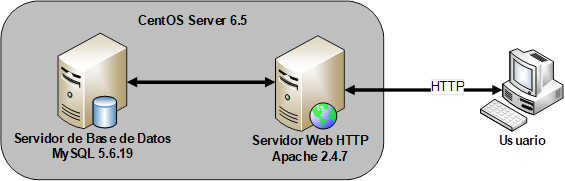
\includegraphics[width=0.94\linewidth]{images/image02_rherrera}
\figcaption{Arquitectura del sistema de la Facultad de Humanidades. Fuente: Elaboración propia}

\end{minipage}

\end {flushleft}

\spacethreemilis

\textbf{Características de hardware del servidor}

Las especificaciones de hardware del servidor físico donde se encuentra la plataforma web de la Facultad son:

\begin{itemize}
\tightlist
\item
  Procesador: Intel Xeon E5620 2,40GHz
\item
  Capacidad del disco duro: 640 GB
\item
  Capacidad de la memoria RAM: 3 GB
\end{itemize}

\textbf{Servicios Web}

Para agilizar los procesos es necesario comunicarse con las siguientes entidades de la Universidad:

\begin{itemize}
\item
  Departamento de Registro y Estadística (RyE): proporciona la información sobre la inscripción del estudiante en una carrera específica y en un año determinado.
\item
  Sistema Integrado de Información Financiera (SIIF): genera una orden de pago con la información del estudiante (carné, unidad, extensión, carrera) y código del curso que va a ser asignado para recuperación.
\end{itemize}

La comunicación con estas dos entidades se realiza a través de servicios web, utilizando los protocolos SOAP y HTTP.

\spacetwomilis
\spacesixmilis

\begin {flushleft}
\noindent\begin{minipage}[c]{\columnwidth}

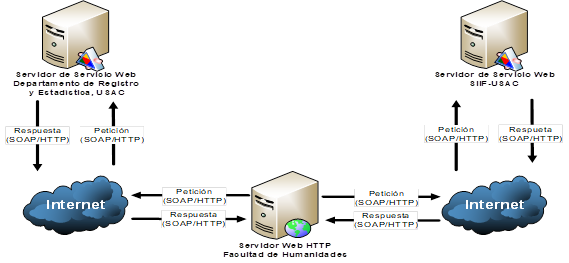
\includegraphics[width=1\linewidth]{images/image03_rherrera}
\figcaption{Diagrama de la conexión a los servicios web de las entidades externas. Fuente: Elaboración propia}

\end{minipage}

\end {flushleft}

\hypertarget{solucion}{%
\subsection{Solución}\label{solucion}}

\spacetwominus

Con base en las necesidades de la Facultad y las herramientas disponibles se establecieron los siguientes objetivos para el proyecto:

\begin{itemize}
\item
  Expeditar la habilitación del pago de recuperaciones en el SIIF.
\item
  Habilitar el portal web de la Facultad para permitir a los estudiantes la asignación a recuperaciones y la generación de las órdenes de pago en línea.
\item
  Automatizar los filtros de asignaciones a las recuperaciones y la confirmación de los pagos respectivos.
\item
  Habilitar el portal web de la Facultad para permitir a los catedráticos el ingreso de notas de recuperaciones en línea, verificando que el valor ingresado sea válido y sin necesitar ingresar la zona.
\end{itemize}

El proyecto se integró a la plataforma web ya existente y se ampliaron sus funcionalidades, de manera que las tareas realizadas manualmente se ejecutan automáticamente y en menor tiempo.

Una vez implementado el proyecto, el proceso tuvo los siguientes cambios:

\textbf{Habilitación de pagos}

La habilitación del pago de recuperaciones en el SIIF se realiza con ayuda del portal web. El sistema determina con los parámetros ingresados qué cursos deben estar disponibles para la generación de orden de pago de recuperaciones. La ejecución de este proceso dura ahora aproximadamente 5 minutos.

\textbf{Asignación }

\begin{itemize}
\item
  El estudiante ingresa con su usuario al portal de la Facultad y selecciona las recuperaciones a asignar.
\item
  El sistema filtra las opciones de manera que el estudiante solo se podrá asignar las recuperaciones a las que tenga derecho.
\item
  Antes de generar la orden de pago se comprueba que el estudiante esté inscrito en dicha carrera durante el año actual a través del servicio web proporcionado por el RyE.
\item
  La orden de pago de las recuperaciones seleccio-
  nadas se generan con el servicio web brindado por SIIF.
\end{itemize}

\textbf{Confirmación de pagos}

\begin{itemize}
\tightlist
\item
  Un servicio web en el sistema de la Facultad (desarrollado durante este proyecto) es consumi-
  do por el SIIF, para notificar cuando los pagos son acreditados. Cuando se recibe la notificación del SIIF, se confirma la asignación del estudiante.
\end{itemize}

• El estudiante ya no necesita entregar la constancia de pago, ya que su pago es validado automáticamente por el sistema.

\begin {flushleft}
\noindent\begin{minipage}[c]{\columnwidth}

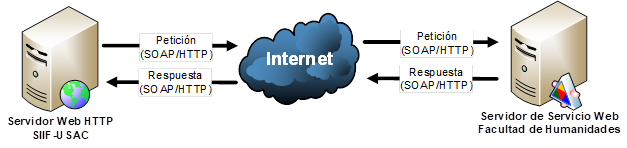
\includegraphics[width=1\linewidth]{images/image04_rherrera}
\figcaption{Diagrama de la conexión del servicio web de la Facultad de Humanidades al SIIF. Fuente: Elaboración propia}

\end{minipage}

\end {flushleft}

\textbf{Ingreso de notas}

\begin{itemize}
\item
  Cuando el catedrático ingresa las notas de la recuperación, el portal verifica que el valor esté en el rango válido y lo asocia a la nota de la zona previamente almacenada en el sistema.
\item
  Las notas son ingresadas al sistema directamente por el catedrático y podrán ser vistas por el estudiante a partir del día siguiente; a diferencia de antes que había que esperar una semana para que las notas fueran procesadas por Control Académico.
\end{itemize}

Se lleva un registro de todas las acciones de los procesos de recuperación ejecutadas en la plataforma web.

\hypertarget{resultados}{%
\subsection{Resultados}\label{resultados}}

Los datos que se muestran a continuación corresponden a las recuperaciones del primer semestre del año 2017.

La cantidad de órdenes de pago generadas en cada recuperación se pueden ver en la siguiente gráfica:

\begin {flushleft}
\noindent\begin{minipage}[c]{\columnwidth}

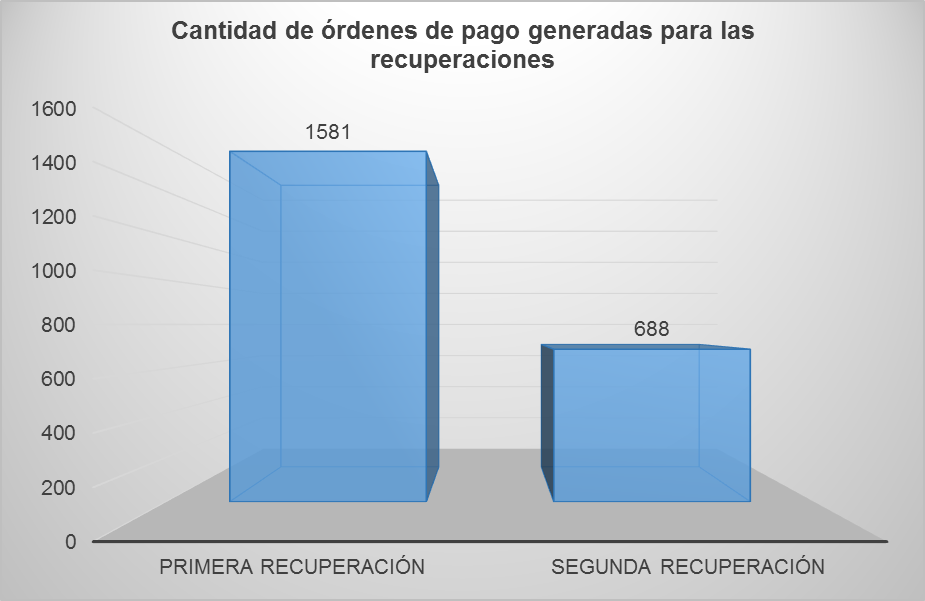
\includegraphics[width=1\linewidth]{images/image05_rherrera}
\figcaption{Cantidad de órdenes de pago generadas para las recuperaciones del primer semestre del año 2017. Fuente: elaboración propia}

\end{minipage}

\end {flushleft}

\spacethreemilis

Los estados finales de las órdenes de pago generadas para la primera recuperación del semestre se pueden ver en la siguiente gráfica:

\begin {flushleft}
\noindent\begin{minipage}[c]{\columnwidth}

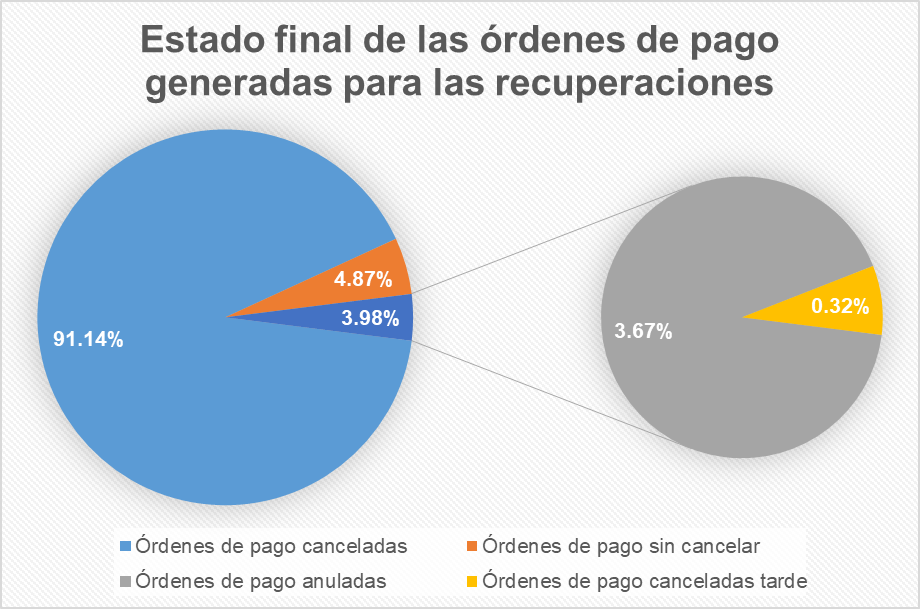
\includegraphics[width=1\linewidth]{images/image06_rherrera}
\figcaption{Estado final de las órdenes de pago generadas para la primera recuperación del primer semestre del 2017. Fuente: elaboración propia}

\end{minipage}

\end {flushleft}

\spacethreemilis

Los estados finales de las órdenes de pago generadas para la segunda recuperación pueden apreciarse en la siguiente gráfica:

\begin {flushleft}
\noindent\begin{minipage}[c]{\columnwidth}

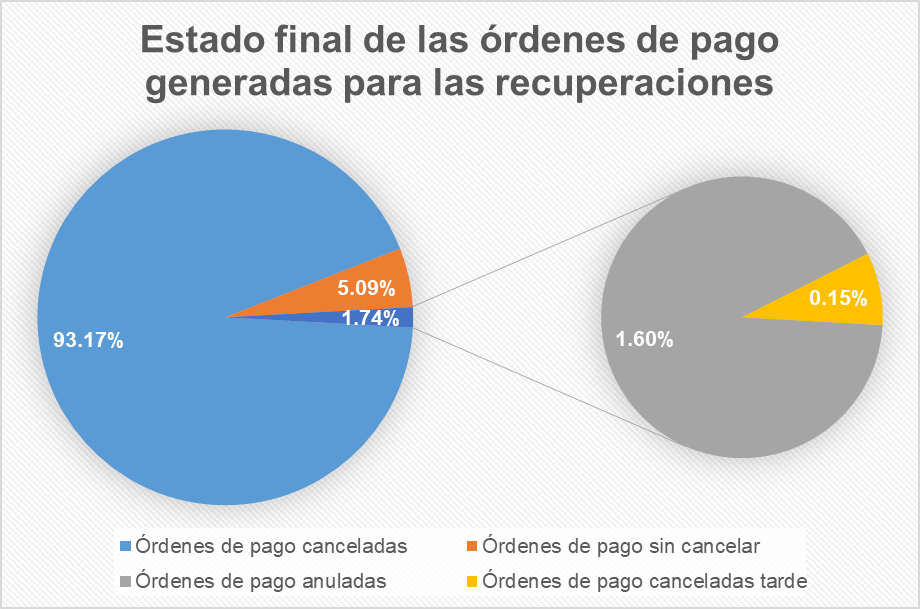
\includegraphics[width=1\linewidth]{images/image07_rherrera}
\figcaption{Estado final de las órdenes de pago generadas para la primera recuperación del primer semestre del 2017. Fuente: Elaboración propia}

\end{minipage}

\end {flushleft}

\hypertarget{conclusiones-2}{%
\section{Conclusiones}\label{conclusiones-2}}

\begin{itemize}
\item
  La implementación de tecnologías de la informa-
  ción en los procesos de recuperaciones es un gran avance para la Facultad de Humanidades, en su propósito de adaptar nuevas opciones tecnológicas para la solución de sus problemas.
\item
  El tiempo para habilitar el pago de las recupera-
  ciones en el SIIF se redujo en un 80\%.
\item
  La asignación y generación de las órdenes de pago de recuperaciones a través de una plataforma web concede un mejor control y orden en dichos procesos.
\item
  La automatización de los filtros de asignación a recuperaciones y la confirmación de pagos conlleva a una ejecución casi inmediata y confiable de los procesos, removiendo al mismo tiempo carga de trabajo al personal de la Facultad.
\item
  El ingreso de notas por medio de una herramienta web mejora la confianza en el proceso, ya que disminuye la información que el catedrático tiene que ingresar, y verifica que las notas estén dentro del rango válido.
\item
  El tiempo en que los estudiantes pueden ver sus notas después de hacer su recuperación se redujo aproximadamente una semana.
\end{itemize}

\hypertarget{discusion-de-resultados}{%
\section{Discusión de resultados}\label{discusion-de-resultados}}

\spaceoneminus
\spacetwominus

La gran cantidad de órdenes de pago generadas muestra la positiva aceptación del proyecto por parte de los estudiantes. Además, la mayor parte de las órdenes de pago generadas fueron canceladas sin ningún inconveniente, lo que significa que el sistema fue lo bastante intuitivo y comprensible como para que los estudiantes pudieran hacer los procedimientos correctamente.

\spacefourminus
\spacetwominus

\hypertarget{recomendaciones-1}{%
\section{Recomendaciones}\label{recomendaciones-1}}

\spacetwominus
\spaceoneminus

A la Unidad de Sistemas de la Facultad de Humanidades:

\begin{enumerate}
\def\labelenumi{\arabic{enumi}.}
\item
  En el futuro, con proyectos similares, se recomienda que su desarrollo sea con base en los productos funcionales del presente proyecto, para que el sistema de la Facultad funcione de manera uniforme.
\item
  Recordar que existe una bitácora en la que están registradas las acciones ejecutadas en los procesos de recuperaciones y puede ayudar a resolver inconvenientes.
\item
  Revisar la bitácora de forma periódica para comprobar si ha habido problemas, como errores de conexión con los servicios web o generación de órdenes de pago fallidas.
\end{enumerate}

\spacefourminus

\hypertarget{referencias-2}{%
\section{Referencias}\label{referencias-2}}

\spacetwominus
\spaceoneminus

\begin{itemize}
\item
  {[}1{]} \href{http://www.repositorio.usac.edu.gt/8239/1/Rodrigo\%20Antonio\%20Herrera\%20De\%20Le\%C3\%B3n.pdf}{Herrera, R.}. \href{https://repositorio.usac.edu.gt}{USAC:} \href{http://www.repositorio.usac.edu.gt/8239/1/Rodrigo\%20Antonio\%20Herrera\%20De\%20Le\%C3\%B3n.pdf}{\emph{Automatización del módulo de Recuperación en la Oficina de Control Académico, Facultad De Humanidades, Universidad De San Carlos De Guatemala}}. Recuperado de: \url{https://bit.ly/3fPKUbq}. {[}Último acceso: noviembre de 2019{]}.
  \spaceoneminus
\item
  {[}2{]} \href{http://scrummethodology.com/}{Desconocido}. \href{http://scrummethodology.com/}{Scrummethodology:} \href{http://scrummethodology.com/}{\emph{Scrum Methodology}}. Recuperado de: \url{https://bit.ly/3gU9qJx}. {[}Último acceso: noviembre de 2019{]}.
\end{itemize}

\spaceoneminus

\begin{itemize}
\tightlist
\item
  {[}3{]} \href{https://www.scrummanager.net/files/scrum_manager.pdf1}{Menzinsky, A., López, G., Palacio, J}. \href{scrummanager.net}{Scrummanager:} \href{https://www.scrummanager.net/files/scrum_manager.pdf1}{\emph{Scrum Master}}. Recuperado de: \url{https://bit.ly/31NJCbW}. {[}Último acceso: noviembre de 2019{]}.
\end{itemize}

\spaceoneminus

\begin{itemize}
\tightlist
\item
  {[}4{]} \href{https://www.centos.org/}{Desconocido}. \href{https://www.centos.org/}{CentOS Project:} \href{https://www.centos.org/}{\emph{The CentOS Project}}. Recuperado de: \url{https://www.centos.org/}. {[}Último acceso: noviembre de 2019{]}.
\end{itemize}

\spaceoneminus

\begin{itemize}
\tightlist
\item
  {[}5{]} \href{https://www.yiiframework.com/}{Desconocido}. \href{https://www.yiiframework.com/}{Yii Framework:} \href{https://www.yiiframework.com/}{\emph{Yii PHP Framework}}. Recuperado de: \url{https://www.yiiframework.com/}. {[}Último acceso: noviembre de 2019{]}.
\end{itemize}

\end {multicols}

\hypertarget{bflorian}{%
\chapter{Vivir y estudiar en Taiwán: La experiencia de un guatemalteco}\label{bflorian}}

\begin {flushleft}

\tcolorboxcommand

\begin{minipage}[c]{3cm}

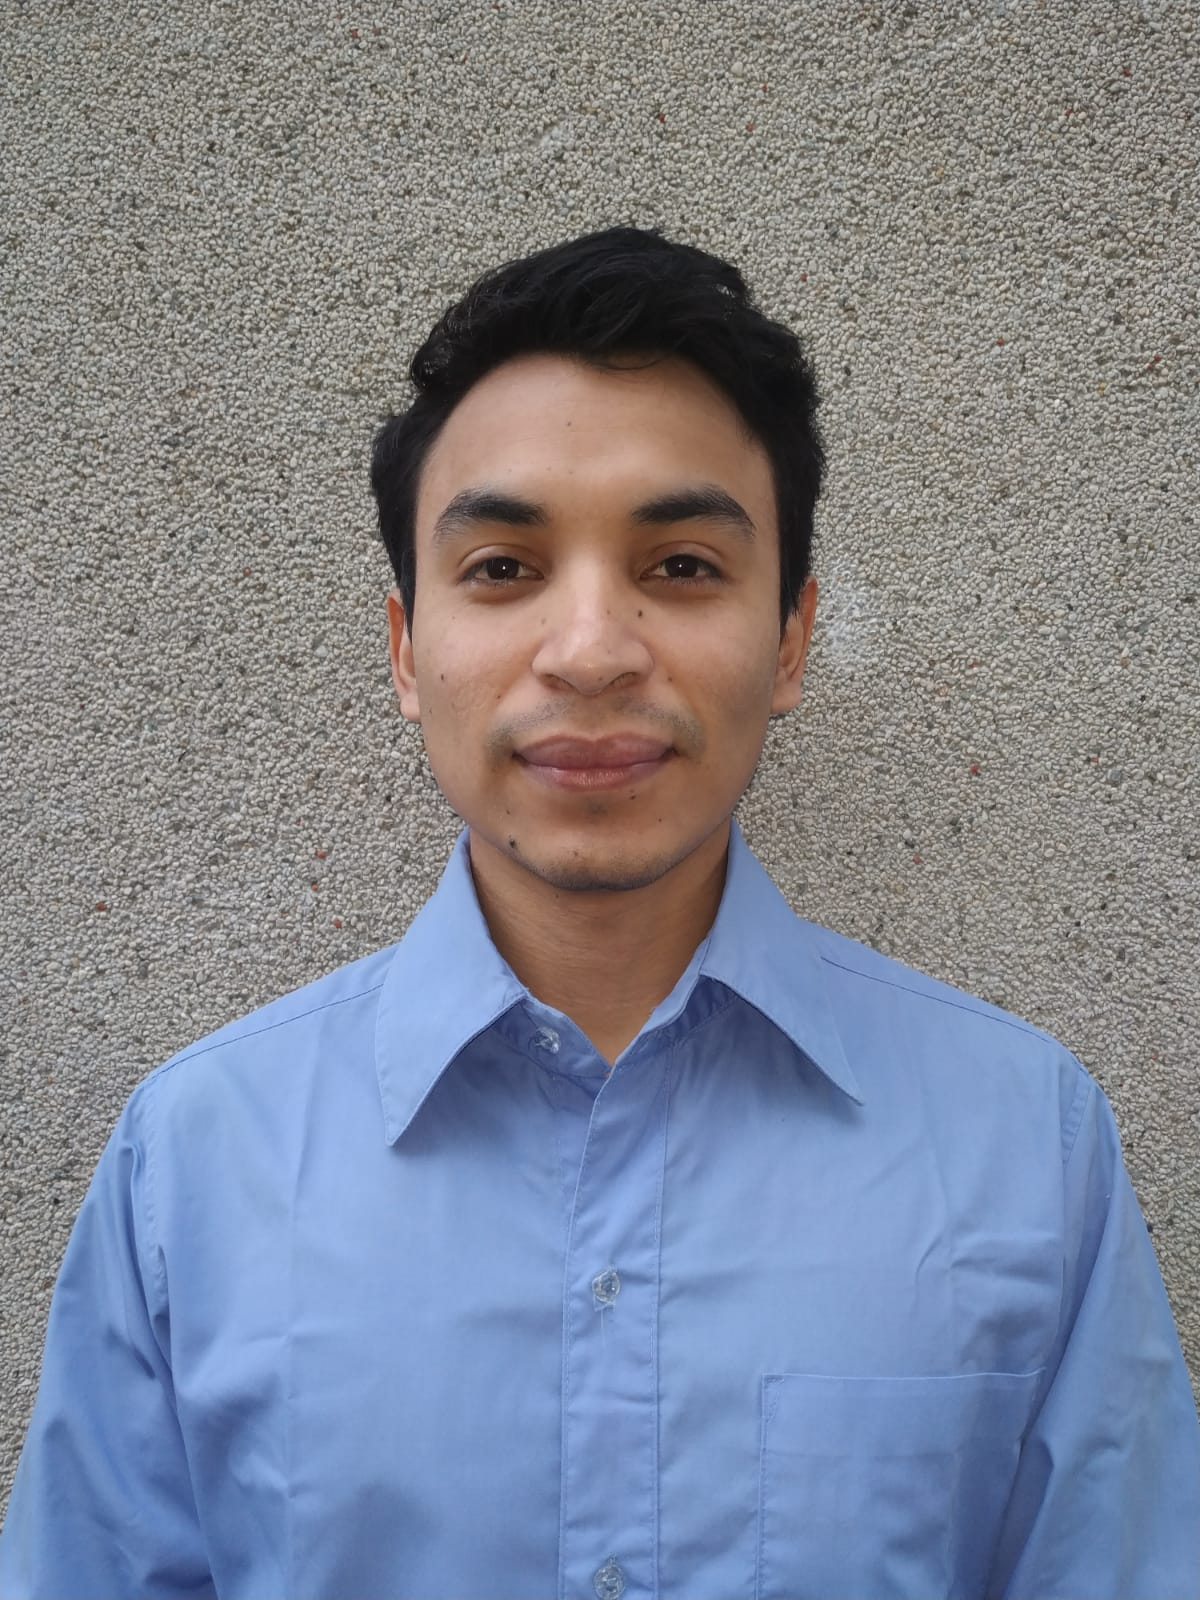
\includegraphics[width=2.5cm,height=\textheight]{images/image01_bflorian1.jpg}

\end{minipage}\begin{minipage}[c]{12cm}

\textbf{Autor:} \emph{Braian Staimer Florián Montenegro}\\
\textbf{Correo electrónico:} \emph{\href{mailto:braianflorian@gmail.com}{\nolinkurl{braianflorian@gmail.com}}}\\
\textbf{Fecha:} \emph{20 de octubre de 2019}

\end{minipage}

\end {tcolorbox}

\end {flushleft}

\hypertarget{resumen-2}{%
\section*{Resumen}\label{resumen-2}}
\addcontentsline{toc}{section}{Resumen}

El presente artículo trata sobre mi experiencia como estudiante de intercambio en la Universidad Nacional Chiao Tung, Taiwán; describo la importancia que tiene este tipo de programas para el crecimiento personal y tecnológico, y cómo impactan dentro de la sociedad; por tanto, se concluye que dichos estudios de posgrado son una realidad y necesidad.

\hypertarget{abstract-2}{%
\section*{Abstract}\label{abstract-2}}
\addcontentsline{toc}{section}{Abstract}

This article is about my experience as an exchange student at National Chiao Tung University, Taiwan; I describe the importance of such programs for personal and technological growth, and how this impacts society. Concluding that it is a reality that postgraduate studies are necessary.

\hypertarget{palabras-clave-3}{%
\section*{Palabras Clave:}\label{palabras-clave-3}}
\addcontentsline{toc}{section}{Palabras Clave:}

\emph{Estudiante, intercambio, programas becarios, extranjero.}

\begin {multicols}{2}

\hypertarget{introduccion-4}{%
\section{Introducción}\label{introduccion-4}}

La Universidad de San Carlos de Guatemala, siendo la rectora de la educación superior de Guatemala, así como otras instituciones, ofrece la oportunidad al estudiante de continuar sus estudios a nivel superior dentro del territorio nacional o en el extranjero. Esto permite que el conocimiento adquirido y la tecnología desarrollada en estos programas de educación puedan ser aplicados en un futuro para resolver problemas que surjan en nuestra comunidad.

\hypertarget{articulo-3}{%
\section{Artículo}\label{articulo-3}}

``Me doy cuenta de que subirme en el avión hacia Taiwán ha sido una de las mejores decisiones de mi vida''.

Desde que era niño, mi familia me ha enseñado principios y valores importantes que me han ayudado como estudiante y como persona, a trabajar intensa-
mente y dar lo mejor de mí para lograr mis objetivos. Durante toda mi vida he disfrutado participar en diferentes actividades, desde formar parte de un equipo de fútbol, hasta ser voluntario en diferentes programas como ``Remodelación de escuelas en el interior del país''; una organización no gubernamental que ayuda a las personas que viven en la pobreza extrema, para que puedan desarrollar sus centros de estudios.

Gracias a estas actividades he adquirido mucha experiencia, nuevos amigos, compartir con líderes y desarrollar diferentes habilidades sociales; así también la posibilidad de estudiar en la mejor universidad de mi país, Universidad de San Carlos de Guatemala, y la oportunidad de viajar a Taiwán, conocer su cultura y vivir la experiencia de realizar un proyecto de investigación en la prestigiosa Universidad Nacional Chiao Tung.

Desde muy joven me interesaron los dispositivos electrónicos, las computadoras, cómo funcionan, cómo están diseñados y construidos, y cómo pueden ser útiles para hacer que nuestras vidas sean más cómodas y convenientes. Para encontrar la carrera que se relaciona con estas materias, investigué un poco y elegí Ingeniería en Ciencias y Sistemas como mi especialidad en la Facultad de Ingeniería. Ahora, después de casi cinco meses de investigar como estudiante de intercambio en el área de Energía, me doy cuenta de que subirme en el avión hacia Taiwán ha sido una de las mejores decisiones de mi vida, y veo claramente qué es lo que quiero seguir aprendiendo y basar mi vida profesional.

El área en la que estoy centrando mi investigación es en cómo controlar el enfriamiento en un entorno de centro de datos utilizando algoritmos de aprendizaje automático, la rama de la ciencias de la computación que, combinando los temas de termodinámica, dinámica de fluidos y transferencia de calor, aborda uno de los mayores desafíos que la humanidad haya enfrentado: la eficiencia energética, el cumplimiento ambiental y aumentar la vida útil de los circuitos integrados que se ven afectados por altas temperaturas en los centros de datos. Cada vez que presionamos un interruptor de luz, manejamos un vehículo, marcamos un número de teléfono, usamos una computadora, o incluso cuando comemos, pensamos en toda la energía que se usó para producir una simple barra de pan, desde el momento que el trigo fue extraído de los campos, transportado y horneado, hasta el momento en que llega a sus manos.

``Después de vivir la experiencia enriquecedora de la Universidad Nacional Chiao Tung durante más de cuatro meses, veo claramente que es el lugar que mejor se adapta a mis necesidades''.

Mi principal objetivo es convertirme en investigador profesional, y después de vivir la experiencia enriquecedora de la Universidad Nacional Chiao Tung durante más de cuatro meses, veo claramente que es el lugar que mejor se adapta a mis necesidades. Sé con certeza que NCTU es donde alcanzaré mis objetivos profesionales, adquiriendo un gran conocimiento de sus profesores y programas docentes de alta calidad; el ranking mundialmente reconocido en los campos de la tecnología, y los recursos de los laboratorios nacionales de clase mundial, el Silicon Valley de Taiwán, el Parque Científico Hsinchu (HSP), reconocido mundialmente, que proporciona instalaciones de investigación a los estudiantes e incluso brinda oportunidades para colaborar con los mejores empresas de alta tecnología y participar en experimentos tecnológicos líderes. Además, tuve la oportunidad de aprender bajo la supervisión de un pionero en Ingeniería Mecánica, con más de doscientos trabajos publicados y más de cuatro mil citas en su área, el profesor Chi-Chuan Wang, con quien tuve la oportunidad aplicar los conocimientos que aprendí en la Universidad de San Carlos de Guatemala, y más importante aún, poder seguir aprendiendo nuevas tecnologías y cómo estas afectan directamente en la industria.

Otro de mis planes es aplicar en mi país el conocimiento aprendido en NCTU, después de completar mi proyecto de investigación. Estoy contento por la oportunidad que se me dio de aportar mi grano de arena para fortalecer el convenio existente entre NCTU y USAC en relación con este tipo de programas de becarios. Espero introducir nuevas tecnologías en el campo de ciencias de la computación, y ser parte de la nueva generación de estudiantes que contribuirá a que nuestra nación se consolide como un país en crecimiento a través del desarrollo de nuevas tecnologías.

\hypertarget{conclusiones-3}{%
\section{Conclusiones}\label{conclusiones-3}}

\begin{itemize}
\item
  Es necesario vivir la experiencia de salir de nuestra zona de confort para descubrir realmente los problemas que vive nuestra sociedad y su posible solución.
\item
  Uno de los retos más difíciles es atreverse a hacerlo, sin embargo, una vez se logra completar este paso, la experiencia será gratificante en todo sentido.
\item
  Cada vez más universidades ofrecen la oportunidad de participar en este tipo de programas de becarios, por lo cual queda claro que cada vez es más necesario continuar elevando nuestro nivel académico.
\end{itemize}

\hypertarget{recomendaciones-2}{%
\section{Recomendaciones}\label{recomendaciones-2}}

\begin{itemize}
\item
  Informarse sobre las oportunidades que ofrecen la Universidad y otras instituciones, ya que cada año son muchas las becas que no se aprovechan.
\item
  Aprender, aprender y seguir aprendiendo, ya que solo nosotros podemos resolver los problemas de nuestra sociedad.
\item
  Dar lo mejor de nosotros para que este tipo de programas pueda continuar, con el afán de que nuestra participación sirva de estímulo para que otros compañeros experimenten estas nuevas vivencias de aprendizaje.
\end{itemize}

\hypertarget{referencias-3}{%
\section{Referencias}\label{referencias-3}}

\begin{itemize}
\item
  {[}1{]} \href{https://www.ugr.es/~filosofia/recursos/innovacion/convo-2005/trabajo-escrito/como-elaborar-un-articulo-cientifico.htm}{Universidad de Granada}. \href{https://www.ugr.es}{Universidad de Granada:} \href{https://www.ugr.es/~filosofia/recursos/innovacion/convo-2005/trabajo-escrito/como-elaborar-un-articulo-cientifico.htm}{\emph{Cómo elaborar un artículo científico}}. Recuperado de: \url{https://bit.ly/30OJ9XF}. {[}Último acceso: noviembre de 2019{]}.
\item
  {[}2{]} \href{https://portal.ingenieria.usac.edu.gt/}{Universidad de San Carlos}. \href{http://www.revistasguatemala.usac.edu.gt/}{Ingeniería, USAC:} \href{http://www.revistasguatemala.usac.edu.gt/index.php/reep/issue/view/90/showToc}{\emph{Revista de la escuela de estudios de postgrado}}. Recuperado de: \url{https://bit.ly/2PMvOcb}. {[}Último acceso: noviembre de 2019{]}.
\end{itemize}

\end {multicols}

\medskip

\HRule

\medskip

\hypertarget{wvaliente}{%
\chapter{Diseño de un colector tipo ciclón de hollín}\label{wvaliente}}

\begin {flushleft}

\tcolorboxcommand

\begin{minipage}[c]{3cm}

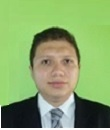
\includegraphics[width=2.5cm,height=\textheight]{images/image01_wvaliente.jpg}

\end{minipage}\begin{minipage}[c]{12cm}

\textbf{Autor:} \emph{Willy Leonel Valiente López}\\
\textbf{Correo electrónico:} \emph{\href{mailto:willyvalientelz@yahoo.com}{\nolinkurl{willyvalientelz@yahoo.com}}}\\
\textbf{Fecha:} \emph{17 de noviembre de 2019}

\end{minipage}

\end {tcolorbox}

\end {flushleft}

\hypertarget{resumen-3}{%
\section*{Resumen}\label{resumen-3}}
\addcontentsline{toc}{section}{Resumen}

El siguiente artículo trata acerca del diseño de un colector tipo ciclón de hollín; se indica inicialmente la situación actual, así como el lugar donde se instalará; seguidamente, se inicia con el proceso de recolección de datos necesarios para el inicio del diseño; posteriormente se realizaron los cálculos del diseño, y por último se los planos isométricos de su potencial instalación.

\hypertarget{abstract-3}{%
\section*{Abstract}\label{abstract-3}}
\addcontentsline{toc}{section}{Abstract}

The following article is about the design of a soot cyclone collector, so it will start indicating the current situation, as well as the place where it will be installed, then it starts with the process of collecting data necessary for the start of the design, subsequently, the design calculations are made, finally, the isometric plans of its potential installation will be made.

\hypertarget{palabras-clave-4}{%
\section*{Palabras Clave:}\label{palabras-clave-4}}
\addcontentsline{toc}{section}{Palabras Clave:}

\emph{Ingeniería de instalaciones, diseño ciclón, hollín.}

\begin {multicols}{2}

\hypertarget{introduccion-5}{%
\section{Introducción}\label{introduccion-5}}

La Facultad de Ingeniería de la Universidad de San Carlos, congruente con su objetivo institucional, permite a los estudiantes hacer su Ejercicio Profesional Supervisado para que apliquen los conocimientos adquiridos durante la carrera y además puedan incursionar en el mercado laboral, lo que los prepara para ejercer su profesión de la mejor manera posible; además, permite hacer un reconocimiento a aquellos trabajos que han demostrado originalidad, aporte personal, nivel profesional, entre otras características en su elaboración; en ese sentido, este trabajo fue reconocido con el premio a la Excelencia del año 2013 categoría graduandos; dicho logro fue gracias a la colaboración del Ingeniero Jaime Batten, con quien logramos formar un equipo de trabajo para su realización; cabe resaltar que sin una buena orientación no se puede llegar muy lejos, es por eso que agradezco al Ingeniero por todo el apoyo brindado, sin el cual no hubiera sido posible obtener dicho reconocimiento.

\hypertarget{articulo-4}{%
\section{Artículo}\label{articulo-4}}

\hypertarget{diagnostico-de-la-situacion-actual}{%
\subsection{Diagnóstico de la situación actual}\label{diagnostico-de-la-situacion-actual}}

Los ciclones son dispositivos de captación de material suspendido en el aire en que la fuerza gravitacional se sustituye con la fuerza centrífuga, dando como resultado una separación de partículas más rápida y con mayor eficiencia; su diseño se basa, normalmente, en familias de ciclones que tienen proporciones bien definidas. Los márgenes de la eficiencia de remoción para los ciclones están con frecuencia basados en las tres familias denominadas: convencional, alta eficiencia y alta capacidad; en ese sentido, para iniciar el diseño del ciclón de hollín es necesario conocer la situación actual, por lo cual en las siguientes figuras se ilustran los planos de las instalaciones de las calderas presentes.

\begin {flushleft}
\noindent\begin{minipage}[c]{\columnwidth}

\centering

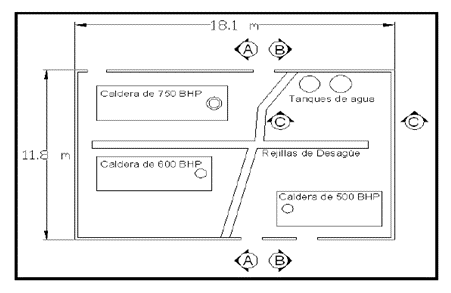
\includegraphics[width=1\linewidth]{images/image02_wvaliente}
\figcaption{Vista de los cortes realizados a la sala de calderas. Fuente: Elaboración propia}

\centering

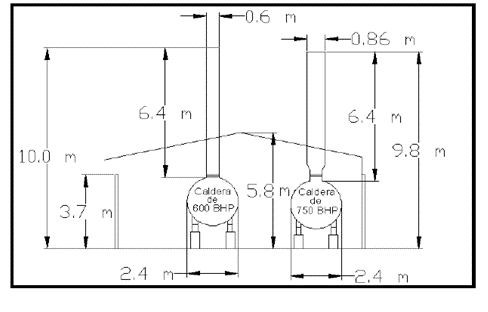
\includegraphics[width=0.82\linewidth]{images/image03_wvaliente}
\figcaption{Corte A. Fuente: Elaboración propia}

\end{minipage}

\end {flushleft}

Seguidamente, se inició con el proceso de aplicación de las cartas de Ringelman, dando como resultado que la densidad aparente visual para cada una de las chimeneas es: 31,50\%, 17,33\% y 19,67\% para las calderas de 500 BHP, 600 BHP y 750 BHP, respectivamente; cabe mencionar, que dichos valores son menores al valor límite (51\%).

\hypertarget{datos-necesarios-para-el-diseno-del-ciclon}{%
\subsection{Datos necesarios para el diseño del ciclón}\label{datos-necesarios-para-el-diseno-del-ciclon}}

Luego de analizar la situación actual, se procedió a la realización del diseño de un colector de hollín tipo ciclón; por lo cual se encontró bibliografía donde se observa la instalación de ciclones en chimeneas de calderas similares a las que posee la empresa, como se observa en la figura 3.

Además, se determinó que era necesario conocer las siguientes variables para el dimensionamiento del ciclón:

\spacefivemilis

\begin{itemize}
\item
  Caudal, presión, viscosidad dinámica, temperatura y densidad de los gases de combustión.
\item
  Tamaño y densidad del hollín.
\item
  Concentración de partículas de hollín en los gases de combustión.
\end{itemize}

\hypertarget{para-conocer-las-variables-mencionadas-se-han-utilizado-las-siguientes-herramientas}{%
\subsection{Para conocer las variables mencionadas, se han utilizado las siguientes herramientas:}\label{para-conocer-las-variables-mencionadas-se-han-utilizado-las-siguientes-herramientas}}

\begin{itemize}
\item
  Tubo de Prandtl y estudio de granulometría.
\item
  Tabla de la densidad y viscosidad del aire en función de la temperatura.
\item
  Peso del hollín y volumen que ocupa en un recipiente cilíndrico.
\end{itemize}

\begin {flushleft}
\noindent\begin{minipage}[c]{\columnwidth}

\centering

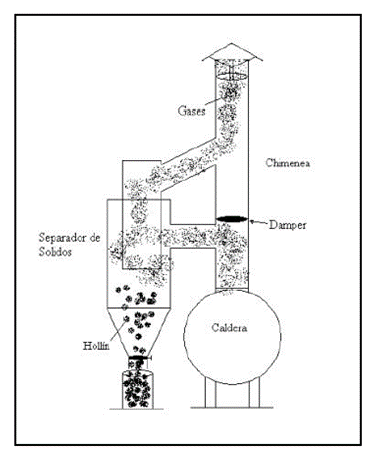
\includegraphics[width=1\linewidth]{images/image04_wvaliente}
\figcaption{Vista de un ciclón instalado en la chimenea de una caldera.}

\end{minipage}

\end {flushleft}

De los requisitos antes mencionados se detallan los más importantes:

\begin{itemize}
\item
  El estudio granulométrico: consiste en conocer el tamaño del grano de hollín; este se desarrolló en el Centro de Investigaciones de Ingeniería (CII);
\item
  El tubo de Prandtl: se construyó para medir las presiones presentes en el gas de descarga: es decir presión estática, dinámica y total; además, para determinar el caudal del gas de descarga se obtendrán dichos datos de la chimenea de la caldera de 750 BHP, porque posee una mayor potencia y diámetro.
\end{itemize}

\begin {flushleft}
\noindent\begin{minipage}[c]{\columnwidth}

\centering

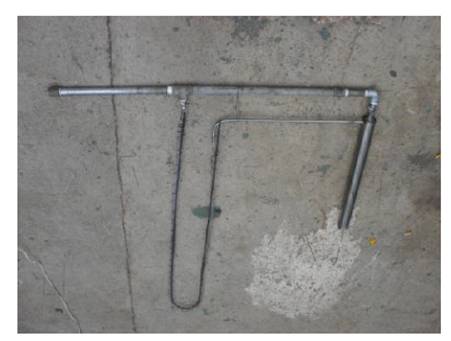
\includegraphics[width=1\linewidth]{images/image05_wvaliente}
\figcaption{Tubo de Prandtl.}

\end{minipage}

\end {flushleft}

Cabe resaltar que se seleccionó el tubo de Prandtl debido a su configuración natural, la cual permite que se inserte momentáneamente en la chimenea.

\begin {flushleft}
\noindent\begin{minipage}[c]{\columnwidth}

\centering

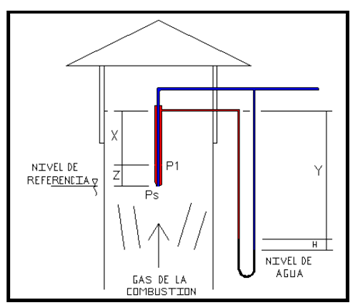
\includegraphics[width=1\linewidth]{images/image06_wvaliente}
\figcaption{Esquema de la utilización del tubo de Prandtl.}

\end{minipage}

\end {flushleft}

\begin {flushleft}
\noindent\begin{minipage}[c]{\columnwidth}

\centering

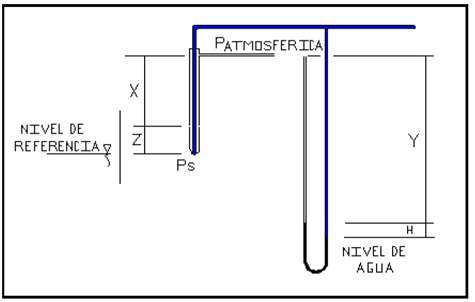
\includegraphics[width=1\linewidth]{images/image07_wvaliente}
\figcaption{Aplicación del tubo de Prandtl para determinar la presión total.}

\end{minipage}

\end {flushleft}

\begin {flushleft}
\noindent\begin{minipage}[c]{\columnwidth}
\centering

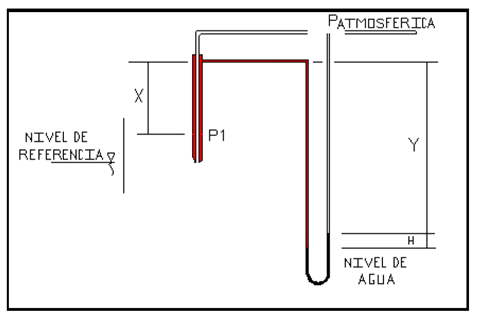
\includegraphics[width=1\linewidth]{images/image08_wvaliente}
\figcaption{Aplicación del tubo de Prandtl para determinar la presión estática.}

\end{minipage}

\end {flushleft}

Para concluir esta sección, en la siguiente tabla se resumen de datos necesarios para el diseño del ciclón.

\begin {flushleft}
\noindent\begin{minipage}[c]{\columnwidth}

\centering

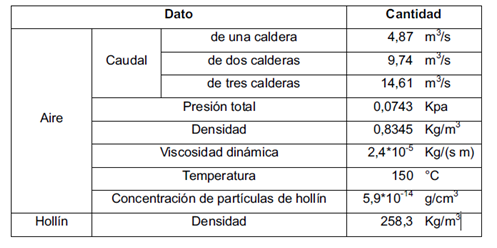
\includegraphics[width=1\linewidth]{images/image09_wvaliente}
\figcaption{Resumen de datos necesarios para el diseño del ciclón.}

\end{minipage}

\end {flushleft}

\hypertarget{procedimiento-para-disenar-un-ciclon}{%
\subsection{Procedimiento para diseñar un ciclón}\label{procedimiento-para-disenar-un-ciclon}}

El procedimiento para diseñar un ciclón es el siguiente:

• Seleccionar el tipo de ciclón, dependiendo del funcionamiento o necesidades requeridas (Tabla 2 y 3).

• Obtener un estimativo de la distribución de tamaño de las partículas en la corriente gaseosa para tratar.

• Calcular el diámetro del ciclón para una velocidad de entrada que esté dentro del intervalo de 15,2 m/s a 27,4 m/s y determinar las otras dimensiones del ciclón con las relaciones establecidas para las familias de ciclones con base en el diámetro.

• Estimar el número de ciclones necesarios para trabajar en paralelo.

\begin {flushleft}
\noindent\begin{minipage}[c]{\columnwidth}

\centering

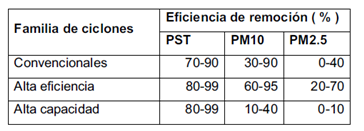
\includegraphics[width=1\linewidth]{images/image10_wvaliente}
\figcaption{Intervalo de eficiencia de diferentes familias de ciclones.}

\spacetenmilis

\centering

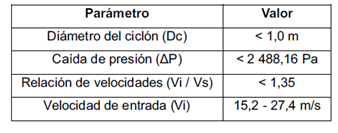
\includegraphics[width=1\linewidth]{images/image11_wvaliente}
\figcaption{Parámetros de diseño para los ciclones de entrada tangencial.}

\end{minipage}

\end {flushleft}

\spacesevenmilis

A partir del conocimiento anterior, se procedió a dimensionar tres ciclones de la siguiente manera: el primero para que trabaje con tres calderas a la vez; el segundo, para que trabaje con dos calderas y el último, para que opere solo con una caldera.

\spacesevenmilis

\begin {flushleft}
\noindent\begin{minipage}[c]{\columnwidth}

\centering

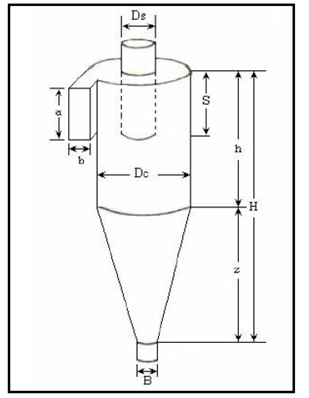
\includegraphics[width=1\linewidth]{images/image12_wvaliente}
\figcaption{Vista de un ciclón.}

\end{minipage}

\end {flushleft}

\spacetenmilis
\spacetenmilis
\spacetenmilis
\spacetenmilis
\spacetenmilis

Al finalizar el dimensionamiento de los tres ciclones, los resultados se ilustran en la tabla 4, donde se muestra un resumen de las principales características y se resalta lo siguiente:

\spacetenmilis

\begin{itemize}
\item
  El mayor diámetro y altura es para el ciclón diseñado para tres calderas.
\item
  La mayor eficiencia la presenta el ciclón diseñado para una caldera.
\item
  Los parámetros del ciclón diseñado para dos calderas se encuentran entre los otros dos ciclones.
\end{itemize}

\begin {flushleft}
\noindent\begin{minipage}[c]{\columnwidth}

\spacetenmilis

\centering

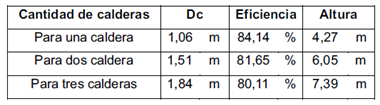
\includegraphics[width=1\linewidth]{images/image13_wvaliente}
\figcaption{Resumen de datos de los ciclones diseñados.}

\end{minipage}

\end {flushleft}

\spacetenmilis

Luego de ver los resultados se estableció que el ciclón que va a utilizarse será el diseñado para dos calderas, debido a que, aun cuando la planta está en expansión, no se considera que en un futuro cercano funcionen las tres calderas simultáneamente; se prevé que solamente lo harán dos.

\spacefivemilis

Finalmente, en las siguientes figuras se muestran los planos propuestos para el cuarto de calderas con el ciclón instalado.

\begin {flushleft}
\noindent\begin{minipage}[c]{\columnwidth}

\centering

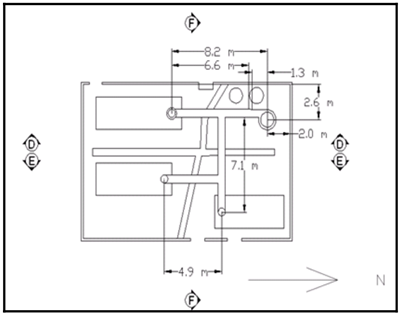
\includegraphics[width=1\linewidth]{images/image14_wvaliente}
\figcaption{Vista en planta de la sala de calderas con ciclón instalado.}

\centering

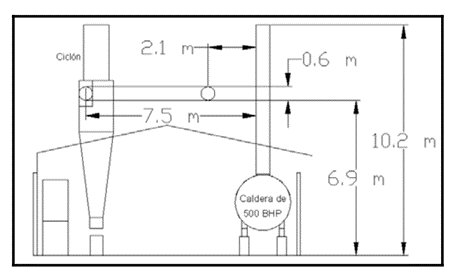
\includegraphics[width=1\linewidth]{images/image15_wvaliente}
\figcaption{Vista del corte F.}

\centering

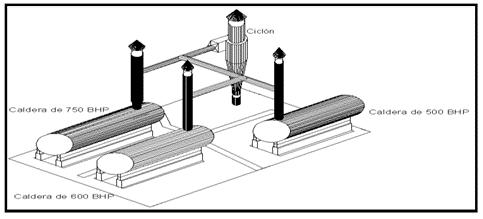
\includegraphics[width=1\linewidth]{images/image16_wvaliente}
\figcaption{Vista isométrica interior del ciclón con conexiones.}

\centering

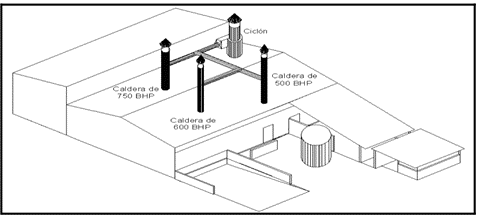
\includegraphics[width=1\linewidth]{images/image17_wvaliente}
\figcaption{Vista isométrica exterior del ciclón instalado.}

\end{minipage}

\end {flushleft}

\hypertarget{conclusiones-4}{%
\section{Conclusiones}\label{conclusiones-4}}

\begin{itemize}
\item
  Se diseñó un colector de hollín tipo ciclón con el cual se pueden trabajar dos calderas, simultáneamente, de la familia de alta captación de tipo Stairmand; de esa manera se podrá reducir el tiempo de limpieza de este al no estar sustrayéndole el hollín continuamente.
\item
  Las características técnicas del colector de hollín son: caudal (9,74 m3/s), velocidad de entrada (15,2 m/s), diámetro mayor (1,51 m).
\end{itemize}

\hypertarget{referencias-4}{%
\section{Referencias}\label{referencias-4}}

\begin{itemize}
\item
  {[}1{]} \href{http://biblioteca.usac.edu.gt/tesis/08/08_0629_MI.pdf}{Valiente, W.(2012)}. \href{http://biblioteca.usac.edu.gt/}{USAC:} \href{http://biblioteca.usac.edu.gt/tesis/08/08_0629_MI.pdf}{\emph{Diseño de un colector tipo ciclón de hollín para las chimeneas de las calderas y plan de contingencia para la Empresa Productos Alimenticios Centroamericanos, S.A. Trabajo de graduación de Ing. Mecánico Industrial. Facultad de Ingeniería, Universidad de San Carlos de Guatemala, 2012. }}. Recuperado de: \url{https://bit.ly/3g1DCl0}. {[}Último acceso: noviembre de 2019{]}.
\item
  {[}2{]} \href{http://www.ingenieroambiental.com/4014/ciclones.pdf}{Echeverry, C. (2006)}. \href{http://www.ingenieroambiental.com/}{Ingeniero Ambiental:} \href{http://www.ingenieroambiental.com/4014/ciclones.pdf}{\emph{Diseño óptimo de Ciclones}}. Recuperado de: \url{https://bit.ly/2Q5O5RL}. {[}Último acceso: noviembre de 2019{]}.
\item
  {[}3{]} \href{http://biblioteca.usac.edu.gt/tesis/08/08_0466_MI.pdf}{López, M. (2008)}. \href{http://biblioteca.usac.edu.gt/}{USAC:} \href{http://biblioteca.usac.edu.gt/tesis/08/08_0466_MI.pdf}{\emph{Montaje, instalación, mantenimiento y principios de operación de una caldera pirotubular de 600 BHP, para la generación y suministro de vapor a una fábrica dedicada a la producción de sopas instantáneas.}}. Recuperado de: \url{https://bit.ly/3gbEFP9}. {[}Último acceso: noviembre de 2019{]}.
\end{itemize}

\end {multicols}

\medskip

\HRule

\medskip

\bibliography{book.bib,packages.bib}

%%%%\printindex




\includepdf{images/contraportada.pdf}


\end{document}
